\chapter{Methodology}

The goal for this research is to investigate the impact of ML methods in STLF. The literature review shows improved accuracy when using ML models. It also highlights the effectiveness of statistical models and SVM's in temporal prediction tasks. It further shows the increased accuracy in ML and AI models, showing how hybrid models can capture the benefits of different models in one. In this section we will focus on the data processing steps, the theoretical background of the models and the methodology followed to produce them.  

\section{Data Collection and Description}
The dataset that is used in the experiments handled in this research was collected by the Panama City government in central America as an initiative to research and improve  methods for short term load forecasting. The dataset is available on Kaggle and  Mendeley Data and provides historical records of electrical load data and relevant weather variables of Panama city\cite{dataset}.

The dataset consists of hourly observations spanning the period from January 2015 to December 2019, yielding approximately 48048 data points. The target variable is the load demand measured in megawatts(MW), while the other features include multiple weather and environmental parameters recorded at different stations across Santiago, Tocumen and David. 

The dataset has the following features as mentioned in \cite{dataset}:
{\small
\begin{itemize}
	\item datetime - The date and time sampled every hour from 
	\item T2M – Temperature at 2 meters above ground (°C)
	\item QV2M – Specific humidity at 2 meters (\%) sampled in the three cities
	\item TQL – Total cloud water content (liters/\si{m^2}) sampled n the three cities
	\item W2M – Wind speed at 2 meters (m/s) sampled in the three cities
	\item Holiday\_ID - a unique value representing a particular holiday in the country
	\item holiday - a binary value representing whether the day is a holiday or not
	\item school - a binary representing schools being open or closed 
	
\end{itemize}
}

The environmental features in the dataset are sampled hourly in the three cities and are represented as toc, san and dav as the extensions of the feature name (e.g. T2M\_dav would be the temperature in David). These meteorological inputs have been selected due to their established influence on electricity demand, as load consumption often correlates with environmental factors such as ambient temperature, humidity, and weather patterns. The relationship between temperature and load has been established with Hor et al \cite{hor2005analyzing} seeing a correlation in the increase in temperature with the increase in the load demand.

The dataset has been cleaned previously by the  initial collectors to ensure minimum erroneous values. The dataset has 4 separate folders namely:
\begin{itemize}
	\item continuous-dataset.csv - containing data sampled every hour for the duration of the collection
	\item test\_dataframes.xslx - a test dataset prepared with historical load from 4 weeks previously \cite{dataset}
	\item train\_dataframes.xslx - a train dataset prepared with historical load from 4 weeks previously with hourly granularity \cite{dataset}
	\item weekly\_pre\_dispatch\_forecast.csv - contains the load forecast from the weekly predispatch report
\end{itemize}

To train the models in this research we chose to use the continuous\_dataset.csv. This is  because of the comprehensive feature set in the dataset. This dataset also has continuous unsplit time series data allowing for testing of custom train test splits that align with the model designs. Finally the flexibility for feature engineering on this dataset is enhanced. It can allow you to generate custom lagged features and rolling statistics giving the researcher transparency and reproducibility.

\section{Data Preprocessing \label{sec:datapreprocessing}}

Data preprocessing is an important step in training of ML and statistical models as it ensures that the data being used is free of noise and outliers. Preprocessing also includes feature engineering which help identify and retain the most influential features, hence simplifying models, reducing redundancy and improving performance \cite{gao2021cooling}.

\subsection{Choice of programming language}
The two options for the programming language to use for this problem were Python and MATLAB. Both these choices offered pros and cons, shown in table \ref{tab:python_matlab_comparison}.
\begin{table}[h!]
	\centering
	\renewcommand{\arraystretch}{1.8} % spacing
	\begin{tabular}{|p{3.5cm}|p{5.5cm}|p{5.5cm}|}
		\hline
		\textbf{Aspect} & \textbf{Python} & \textbf{MATLAB} \\
		\hline
		\textbf{Data Processing} & Rich data processing framework(Pandas, NumPy). & Built-in data handling but less flexible than Python’s frameworks. \\
		\hline
		\textbf{Machine Learning \& AI} & Strong libraries: TensorFlow, PyTorch, Scikit-learn. & ML toolboxes available, but limited adoption compared to Python. \\
		\hline
		\textbf{Community Support} & Huge global community; extensive tutorials, forums, and open-source contributions. & Strong academic/engineering base, but smaller community outside academia. \\
		\hline
		\textbf{Flexibility of production environment} & Works well for online development online with google collab offering CPU and GPU services. & Better integration with control simulations, and hardware prototyping. \\
		\hline
		\textbf{Ease of Use} & Easy-to-read syntax, intuitive for beginners, widely taught. & Powerful for numerical computing syntax less intuitive for general-purpose tasks. \\
		\hline
		\textbf{Performance} & Fast with optimized libraries (NumPy, TensorFlow GPU acceleration). & Highly optimized for matrix operations sometimes faster out-of-the-box for linear algebra. \\
		\hline
	\end{tabular}
	\caption{Comparison of Python and MATLAB for data analysis and machine learning.}
	\label{tab:python_matlab_comparison}
\end{table}

Matlab is powerful in numerical computing and is widely used in academia and engineering settings, python was chosen for this research due to several key reasons. Python provides robust data processing frameworks, which make data cleaning, transformation and preprocessing efficient and straightforward. Python supports industry standard ML frameworks such as TensorFlow and Scikit-learn that were extensively used in this research for setting up and training the models. These models offer a ease of use and advanced modeling and experimentation. Python has a massive global community offering more resources and troubleshooting support more than MATLAB. After careful consideration of the pros and cons, python was used for modeling.

\subsection{Feature Engineering}
The data handling framework that is used in the project is python Pandas. Pandas offers a wide range of processes to feature engineer your dataset. It also sets the dataset into a format that is user friendly for training and testing both statistical and machine learning models. 

\paragraph{Forward Filling}
The first step taken to ensure that the dataset is complete and there are no missing values, was the forward fill method. Forward fill is a method where you fill a missing value with the last known value. The last known value is carried forward to replace the missing value. An illustration of how this method works is shown in figure \ref{fig:forward_fill}. This method is simple and effective for filling in values such as temperature which have low variance. 

\paragraph{Day of Week Encoding}
A \texttt{day\_of\_week} column was added to the dataset to represent the weekday on which each observation occurred. This feature allows the models to capture temporal seasonality related to human activity patterns that typically vary across weekdays and weekends. For instance, energy consumption or cooling demand may be systematically higher on weekdays compared to weekends.
\paragraph{Cyclical Encoding : } To avoid discontinuities and ensure the network learns smooth transition of time eg from 11PM to 12 AM , cyclical encoding is applied to hour, day of week and month. With cyclical encoding the times 11PM and 12AM are represented as being close to each. This is performed by using sine and cosine transformation to the dataset columns associated.

\paragraph{Weekend and Weekday Tag}
Building on the day-of-week information, a binary tag distinguishing between weekdays and weekends was introduced. This feature reduces the dimensionality of temporal effects and allows the models to easily account for systematic differences in behaviour between weekdays and weekends.

\paragraph{Month Identifier}
To incorporate longer-term seasonal variations, a \texttt{month} identifier was added. This feature makes it possible to detect monthly or seasonal cycles in the data, such as weather-related patterns or operational schedules that repeat on a monthly basis.

\paragraph{Holiday Combination Feature}
The dataset included two holiday-related variables: \texttt{holiday\_ID}, which was a categorical value ranging from 1 to 22 representing different types of holidays, and \texttt{holiday}, which was a binary value indicating whether a given day was a holiday or not. To enhance the usability of these features, a combined feature was created by multiplying \texttt{holiday\_ID} with \texttt{holiday}. This ensured that non-holiday days were represented as zero, while holidays retained their unique identifiers. This transformation simplified model training by consolidating redundant information into a single, more informative feature.

\subsection{Outlier Detection and Removal using the Hampel Identifier Method \label{sec:HI_method}}
Outliers can significantly bias statistical and machine learning models if not properly addressed. To mitigate this, the Hampel identifier(HI) method was employed for outlier detection. The HI method was chosen because it is a robust statistical technique based on the median and the median absolute deviation (MAD)\cite{hiceemdanQteg}. The method is also robust to heavy tailed data and skewed distributions of raw data. Below are the equations used for the implementation as taken from \cite{hiceemdanQteg}.

Consider the input sequence \(A = [a_1, a_2, \ldots, a_k]\). For each sample \(a_i\), a symmetric sliding window of length \(w = 2n + 1\) centered at \(i\) is defined. Within this window:

\[
m_i = \operatorname{median}(a_{i-n}, \ldots, a_i, \ldots, a_{i+n})
\tag{1}
\]

The median absolute deviation (MAD) is calculated as:

\[
\mathrm{MAD}_i = \operatorname{median}\big(|a_{j} - m_i| : j \in [i-n,\, i+n]\big)
\tag{2}
\]

To estimate the standard deviation, the MAD is scaled using a constant \(\alpha = 0.6745\) (consistent with normal distribution assumptions):

\[
\sigma_i = \frac{\mathrm{MAD}_i}{\alpha}
\tag{3}
\]

An observation is identified as an outlier if it deviates from the local median beyond three times the estimated standard deviation:

\[
|a_i - m_i| > 3\sigma_i
\tag{4}
\]

If an outlier is detected, the original value \(a_i\) is replaced with the local median \(m_i\). This correction preserves the temporal structure of the data while reducing the influence of anomalies. Incorporating HI ensures that erroneous spikes caused by equipment errors, missing sensor calibration, or human errors do not affect model training and forecasting. This HI formulation was shown to improve quality of raw data and reduce the occurrence of spikes in the data \cite{hiceemdanQteg}.

\subsubsection{Data Normalization}

To ensure that the features contributed proportionally during model training, all numerical variables in the dataset were normalized, with the exception of the \texttt{datetime} column, which was retained in its original format for temporal referencing and indexing the dataset. Normalization prevents features with larger absolute values from dominating those with smaller ranges, and it improves the convergence behavior of machine learning algorithms.

Several normalization and standardization approaches exist, such as z-score standardization, robust scaling, and Min–Max scaling. In this work, the Min–Max scaling method was used due to its effectiveness in re-scaling features to a fixed range while preserving the original distribution’s shape. The transformation is defined as:

\[
x' = \frac{x - x_{\min}}{x_{\max} - x_{\min}}
\tag{5}
\]

where \(x\) is the original feature value, \(x_{\min}\) and \(x_{\max}\) are the minimum and maximum values of the feature, and \(x'\) is the normalized value re-scaled to the interval \([0,1]\).

The Min–Max scaling method was chosen because it is well-suited for neural networks and distance-based models, particularly those relying on gradient descent, as these algorithms perform optimally when features are restricted to a bounded range \cite{featureScaling}. Unlike z-score normalization, which re-centers data around the mean, Min–Max scaling preserves the original relative spacing between values, making it appropriate when proportional differences carry meaning. Furthermore, by rescaling all features to the interval \([0,1]\), it provides a consistent and interpretable representation that simplifies visualization and ensures that all features contribute fairly during training.

By applying Min–Max scaling, the dataset was transformed into a consistent format across all features, thereby improving model training stability and ensuring fair contribution of each feature to the learning process.


The steps taken for the data preprocessing are shown in the fig \ref{fig:preprocessing_steps_flowchart} in appendix   \ref{sec:appendixA}. 

\section{Evaluation Metrics \label{sec:eval_metrics}}
The models were compared using standard error metrics and information criteria that are widely used in forecasting literature. These metrics provide complementary views on model performance in terms of accuracy, error magnitude, and model complexity. The chosen metrics are briefly described below. 

\subsubsection{Mean Absolute Percentage Error (MAPE)} 
MAPE expresses forecast accuracy as a percentage, making it easy to interpret across different scales. Lower values indicate better performance.  
\[
\text{MAPE} = \frac{100}{n}\sum_{t=1}^{n} \left| \frac{Y_t - \hat{Y}_t}{Y_t} \right|
\tag{6}
\]

\subsubsection{Mean Squared Error (MSE)} 
MSE penalises larger errors more heavily by squaring them, making it sensitive to outliers.  
\[
\text{MSE} = \frac{1}{n}\sum_{t=1}^{n} (Y_t - \hat{Y}_t)^2
\tag{7}
\]

\subsubsection{Root Mean Squared Error (RMSE)} 
RMSE is the square root of MSE and brings the error measure back to the same scale as the original data.  
\[
\text{RMSE} = \sqrt{\frac{1}{n}\sum_{t=1}^{n} (Y_t - \hat{Y}_t)^2}
\tag{8}
\]

\subsubsection{Coefficient of Determination ($R^2$)} 
$R^2$ measures how well the forecasts explain the variance in the actual data. Higher values (closer to 1) indicate better fit.  
\[
R^2 = 1 - \frac{\sum_{t=1}^{n} (Y_t - \hat{Y}_t)^2}{\sum_{t=1}^{n} (Y_t - \bar{Y})^2}
\tag{9}
\]

\subsubsection{Akaike Information Criterion (AIC)} 
AIC balances model fit and complexity. It penalizes over-parameterized models, with lower values indicating a better trade-off.  
\[
\text{AIC} = 2k - 2\ln(\hat{L})
\tag{10}
\]
where $k$ is the number of model parameters and $\hat{L}$ is the maximized likelihood.



\section{Statistical and Machine Learning Models}
\subsection{Exponential Smoothing}

Exponential smoothing has been widely used in STLF due to its low computational needs and fast processing times. The core idea of this method is to produce a forecast from an exponentially weighted average of past observations, giving the largest weight to the most recent data and exponentially decreasing weights to older data \cite{ostertagova2011simple}. This method's functionality has been discussed extensively in section \ref{sec:exponential smoothing}. In this section we will focus on the theoretical fundamentals and the choice of model we used in our research.  

There are multiple forms of ES, each designed to capture different components of a time series data.
\paragraph{Simple Exponential Smoothing(SES)}\label{par:ses}
SES is designed for time series datasets that lack seasonality and trend. The forecast is based solely on the weighted average of past observations. If $\hat{Y}_{t}$  is the value at time t  and $\alpha$ is the smoothing parameter between 0 and 1. The equation for the smoothed value $S_{t}$ would be \ref{eqn:6} as adapted from \cite{ostertagova2011simple}.

\[
\hat{S}_{t+1}  = \alpha Y_t + (1-\alpha)\hat{Y}_t
\tag{11}
\label{eqn:6}
\]
 Though the simplicity of SES is good for very low computational tasks, it is not favorable because of its low accuracy and failure to identify presence of the trend and seasonality in the data.
 
 \paragraph{Double Exponential Smoothing (DES)} method introduces capturing of trend in the time series data. This is in addition to the already existing level component in SES \ref{par:ses}. The equation of DES as adapted from \cite{nist_double_exp_smoothing} would be:
 \[
  S_t = \alpha Y_t + (1-\alpha)(S_{t-1} + b_{t-1})
  \tag{12}
 \label{eqn:7}
 \] 
 \[
  b_t = \gamma (S_t - S_{t-1}) + (1-\gamma) b_{t-1}
  \tag{13}
 \label{eqn:8}
 \]
 
 where $b_t$ would be the estimated trend or slope of the dataset and $\gamma$ would be the smoothing parameter for the trend  between 0 and 1. The data used in this research shows a clear flat trend over the long-term and seasonality every 24 hours with a fast rise and peak demand during midday shown in image \ref{fig:weeklydemand}. This 24 hour seasonality brings us to the third ES model which is the Triple Exponential Smoothing (TES). 
 \begin{figure}[h]
 	\centering
 	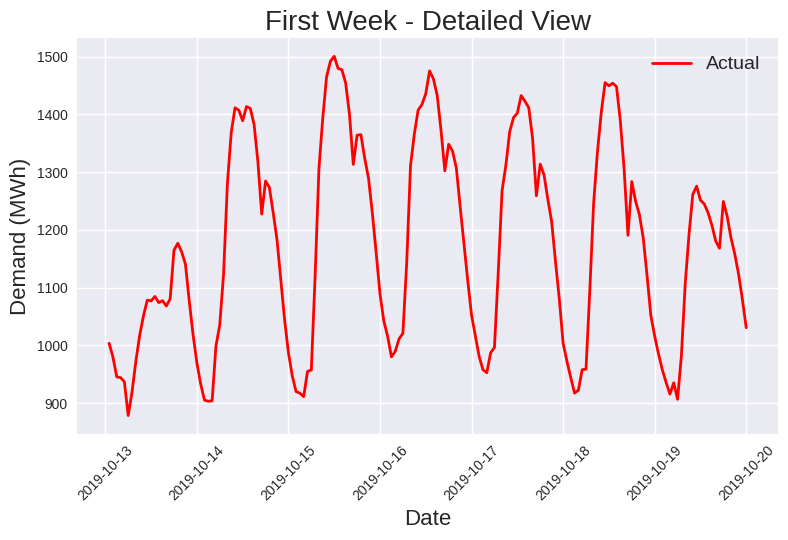
\includegraphics[width=0.7\linewidth]{Chapters/images/weekly_demand}
 	\caption{Real electricity demand from Sunday 13th to Saturday 20th of October 2019}
 	\label{fig:weeklydemand}
 \end{figure}
 
 \paragraph{Triple Exponential Smoothing }introduces the equation that takes care of the seasonality component \cite{nist_double_exp_smoothing}. TES inherits equation \ref{eqn:7} and \ref{eqn:8} and introduces equation \ref{eqn:9} for seasonality adapted from \cite{nist_double_exp_smoothing}.
 \[
 I_t = \beta \frac{Y_t}{S_t} + (1-\beta) I_{t-m}  
 \tag{14}
 \label{eqn:9}
 \]
 $I_t$ is the estimated seasonal component and $\beta$ is the seasonality constant that is between 0 and 1. With the combination of equation \ref{eqn:6} , \ref{eqn:8}  and \ref{eqn:9} the overall smoothed value equation would be \ref{eqn:10}. 
 \[
 S_t = \alpha \frac{Y_t}{I_{t-L}} + (1-\alpha)(S_{t-1}+b_{t-1})
 \tag{15}
 \label{eqn:10}
 \]
 
 \paragraph{Damping} is a mechanism used to reduce or dampen the trend in forecasts over long horizons \cite{taylor2003exponential}. This method makes the forecast trend more conservative, preventing it from overshooting the actual data, which is a common problem in ES methods projecting a linear trend indefinitely in the future \cite{taylor2003exponential}. The equation below is for the smoothed value inclusive of the damping factor $\phi$ which is between 0 and 1, adapted from \cite{taylor2003exponential}. With equation \ref{eqn:11.a} being the additive in level and equation \ref{eqn:11.b} being the multiplicative in level.
 \[
 	S_t = \alpha \frac{Y_t}{I_{t-L}} + (1-\alpha)\bigl(S_{t-1} + \phi\, b_{t-1}) 
 \tag{16}
 \label{eqn:11.a}
 \] 
 \[
 S_t = \alpha \frac{Y_t}{I_{t-L}} + (1-\alpha)\bigl(S_{t-1} \cdot b_{t-1}^{\,\phi}\bigr)
 \tag{17}
 \label{eqn:11.b}
 \]
 

 \subsubsection{Choice of best Exponential Smoothing model}
 ES was used as a benchmark for testing the ML models. However because of the different variations of ES an algorithm was  developed to help choose the best performing ES model for the research. The models performance were compared on their MAPE, MAE, Mean Squared Error(MSE), RMSE and the AIC.
 
 This algorithm would create a model using \textit{statsmodel holtwinters} \cite{statsmodels_expsmoothing_doc} and test  performance of forecasts o. Different model's performance would be compared to each other. Image \ref{fig:exponential-smoothing-model-choice} in appendix A shows a the algorithm followed to choose the best ES model. Table \ref{tab:es_model_selection} shows the different models that were tested to find the best model.

\begin{table}[ht]
	\centering
	\resizebox{\textwidth}{!}{%
		\begin{tabular}{lccccccc}
			\hline \\
			\textbf{Model} & \textbf{Trend} & \textbf{Seasonality} & \textbf{Seasonality Period} & \textbf{Damped} & \textbf{MAPE (\%)} & \textbf{MSE (MWh)} & \textbf{AIC}
			 \\
			\hline
			Simple               & None  & None & –  & No  & 13.76\%  & 180.98 & 343990.96 \\
			Double               & Add   & None & –  & No  & 15.14\%  & 172.11 & 327001.68 \\
			Triple\_Add          & Add   & Add  & 24 & No  & 10.56\%  & 125.56 & 277981.02 \\
			Triple\_Mul          & Mul   & Mul  & 24 & No   & 34.48\%  & 408.23 & 272265.85 \\
			Triple\_Add\_Damped  & Add   & Add  & 24 & Yes &  9.99\%  & 120.81 & 277708.98 \\
			Triple\_Mul\_Damped  & Mul   & Mul  & 24 & Yes & 10.01\%  & 119.49 & 272266.18 \\
			\hline
		\end{tabular}%
	}
	\caption{Exponential Smoothing Models chosen for benchmarking and their performance.}
	\label{tab:es_model_selection}
\end{table}

Comparison of performance metrics through the algorithm in figure \ref{fig:exponential-smoothing-model-choice} was the Triple Multiplicative Damped algorithm with a seasonality period of 24 data points. Since the dataset is sampled hourly the seasonality was set to 24 hours. The MAPE and MSE are very close to each other with a difference of about 0.01 each. However the AIC value for  $Triple\_Mul\_Damped$ is lower than the one for $Triple\_Add\_Damped$, this showing a better model fit for  $Triple\_Mul\_Damped$. The final choice for the ES model was  $Triple\_Mul\_Damped$ and it served as a benchmark for testing performance of other models used in the experiment.
\subsubsection{Implementation of the Triple Multiplicative Damped ES model}



\subsection{Deep Belief Network}
 
 A DBN is a probabilistic generative model composed of multiple layers of stochastic, latent variables \cite{zhang2017deep}. It is constructed by stacking multiple layers of RBMs on top of each other \cite{zhang2016short}. This model benefits from its capabilities of limiting the occurrence of the local minima by pre-training RBMs using unsupervised training to adjust weights and parameters to ensure an enhanced performance in actual prediction use cases.
 
\subsubsection{Restricted Boltzmann Machine (RBM)}

A Restricted Boltzmann Machine (RBM) is a two-layer probabilistic generative model designed to learn the underlying probability distribution of input data. RBMs are widely used as building blocks for constructing DBNs \cite{dong2021short}. The architecture consists of a \textit{visible layer}, which receives the observed data, and a \textit{hidden layer}, which captures latent features and higher-order correlations in the data. Learning in RBMs is unsupervised, the model attempts to represent the structure of the input data by adjusting its parameters weights and biases so as to maximize the likelihood of the training samples \cite{zhang2017deep}.

An RBM is defined by a weight matrix that connects each visible unit to each hidden unit in a bipartite manner, together with bias vectors for both layers. No intra-layer connections are permitted, which simplifies inference and training. The structure is shown in figure \ref{fig:singlerbm}, adapted from Zhang et al. \cite{zhang2017deep}.

\begin{figure}[ht]
	\centering
	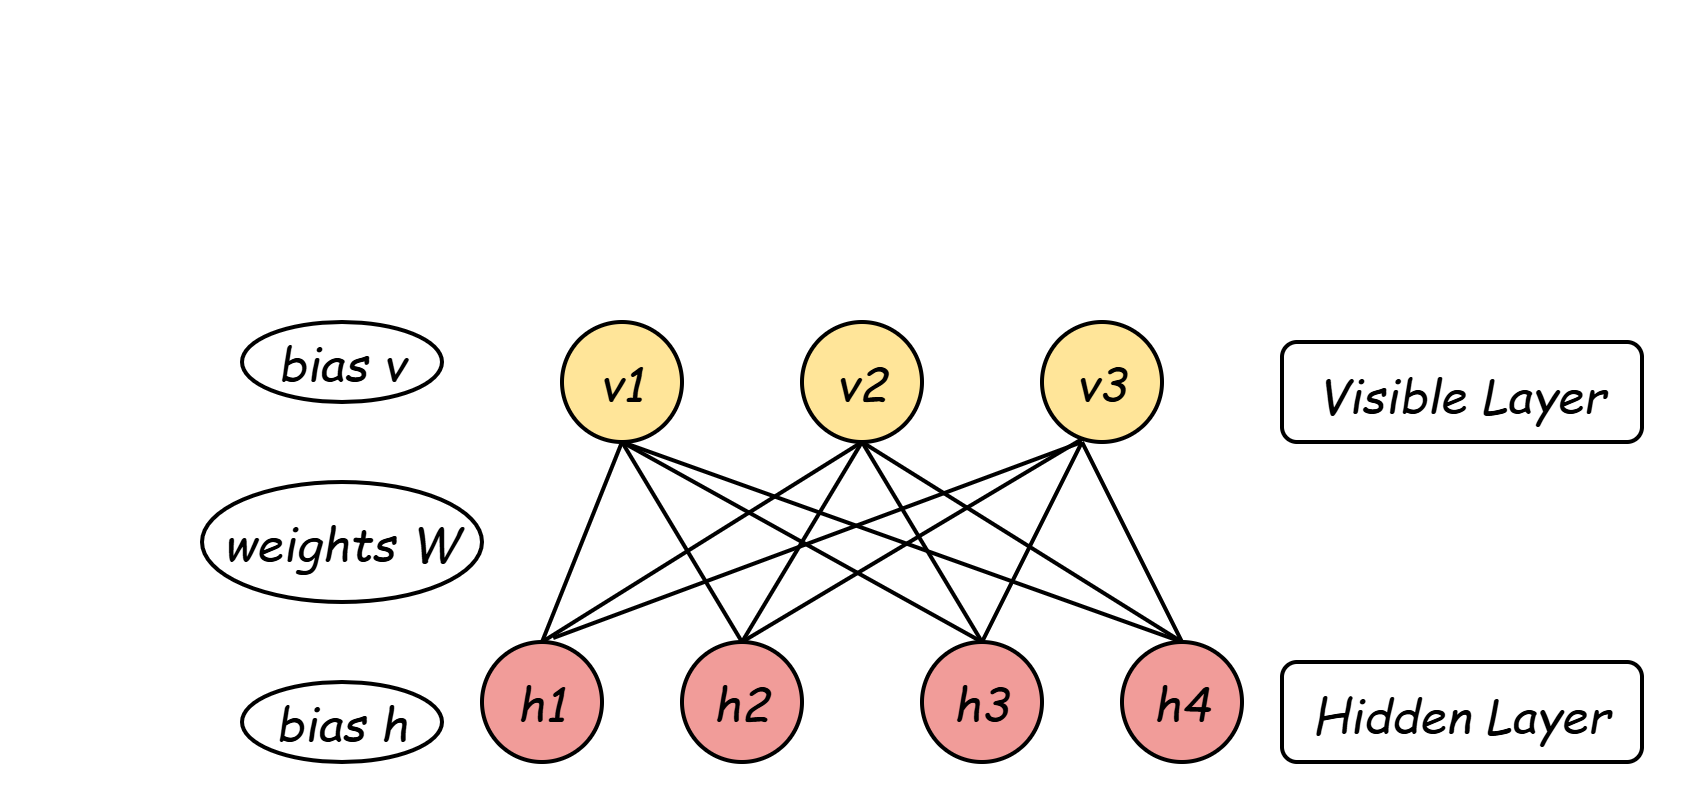
\includegraphics[width=0.7\linewidth]{Chapters/images/singleRBM}
	\caption{Illustration of an RBM with visible and hidden layers, including weights and biases}
	\label{fig:singlerbm}
\end{figure}

\paragraph{Energy-Based Formulation: } 
An RBM is an energy-based model, meaning it assigns a scalar energy value to each configuration of visible and hidden units. Configurations with lower energy are more likely under the model. The energy function is given by \cite{kong2019improved, zhang2016short}:

\[
E(v,h;\theta) = -\sum_i a_i v_i - \sum_j b_j h_j - \sum_{i,j} v_i W_{ij} h_j
\tag{18}
\label{eqn:12}
\]

where
\begin{itemize}
	\item $v_i$: the state of visible unit $i$,
	\item $h_j$: the state of hidden unit $j$,
	\item $a_i$: the bias associated with visible unit $i$,
	\item $b_j$: the bias associated with hidden unit $j$,
	\item $W_{ij}$: the weight between visible unit $i$ and hidden unit $j$,
	\item $\theta = \{W, a, b\}$: the model parameters.
\end{itemize}

\paragraph{Probability Distribution: } 
Using the energy function, the joint probability of a visible hidden configuration is defined by the Boltzmann distribution \cite{DBN_GeeksforGeeks}:

\[
P(v,h) = \frac{e^{-E(v,h)}}{Z}
\tag{19}
\label{eqn:13}
\]

where $Z$ is the \textit{partition function}, given by summing over all possible visible and hidden states:
\[
Z = \sum_{v,h} e^{-E(v,h)}
\tag{20}
\]

The probability of a visible vector $v$ is obtained by marginalizing out the hidden layer:
\[
P(v) = \frac{1}{Z} \sum_{h} e^{-E(v,h)}
\tag{21}
\]

\paragraph{Training RBMs:} 
RBMs are typically trained using the \textit{Contrastive Divergence} (CD) algorithm which is a version for forward and back propagation. Training consists of two phases:

\begin{enumerate}
	\item \textbf{Positive phase:} a visible layer vector from the data activates the hidden layer, and correlation outputs $\langle v_i h_j \rangle_{\text{data}}$ are computed.
	\item \textbf{Negative phase:} the hidden units output are used to reconstruct the visible layer, producing a reconstructed vector. From this, correlations $\langle v_i h_j \rangle_{\text{recon}}$ are obtained.
\end{enumerate}

The difference between the two phases which is error provides the learning signal for updating weights:
\[
\Delta W_{ij} = \eta \Big( \langle v_i h_j \rangle_{\text{data}} - \langle v_i h_j \rangle_{\text{recon}} \Big)
\tag{22}
\label{eqn:14}
\]
where $\eta$ is the learning rate. In this way, the RBM iteratively learns to reduce the gap between the distribution of the training data and the distribution it models. The feed-forward (data-to-hidden) and feed-backward (hidden-to-reconstruction) passes, together with weight updates, constitute the CD training loop \cite{RBM_GeeksforGeeks}.

\paragraph{DBN (Stacked RBMs)} When 1 or more RBMs are stacked together they create a DBN. This DBN has the advantage of pre-trained RBMs that have adjusted their weightings to minimize error in the training phase. Stacking of RBMs is as shown in the figure \ref{fig:correctrbm}.
\begin{figure}[h]
	\centering
	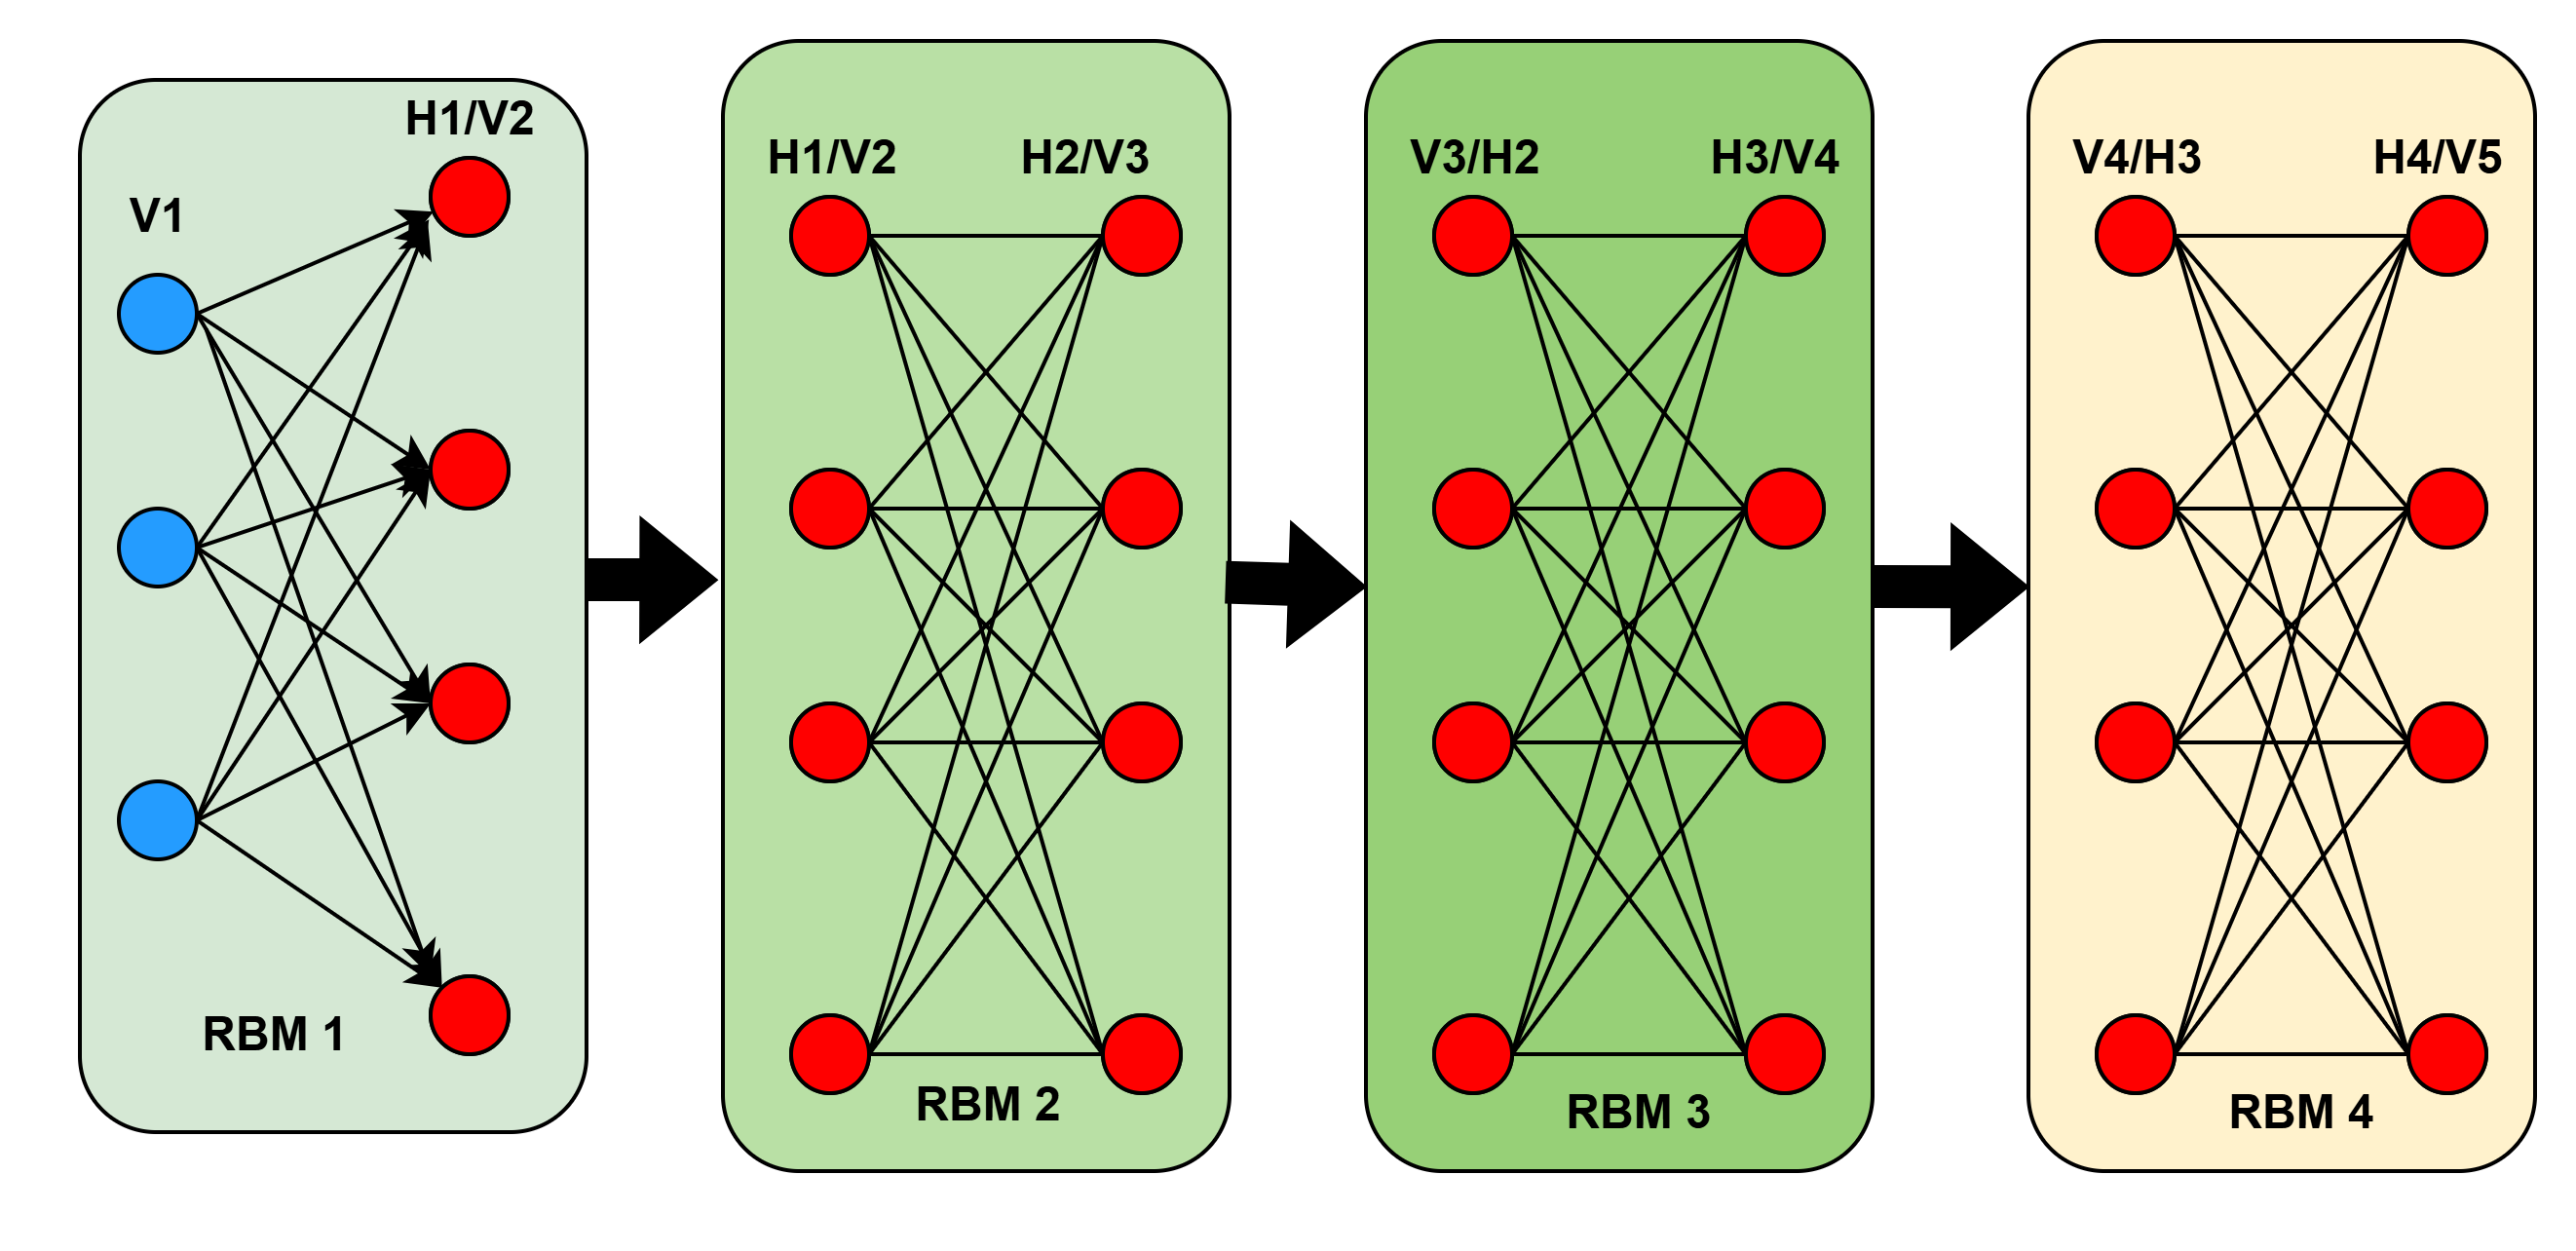
\includegraphics[width=0.7\linewidth]{Chapters/images/CORRECT_RBM}
	\caption{An illustration of stacked RBMs making a DBN}
	\label{fig:correctrbm}
\end{figure} 
This illustration highlights how the hidden layer of the first RBM is the visible layer of RBM 2. During pretraining each RBM is trained separately. RBM1 will receive the original data and perform CD on RBM1, the recreated output on the hidden layer 1(HD1) becomes the input of RBM2 through the visible layer 2(V2). RBM2 will go through CD and continues the loop until the full RBM has been trained and the weights have been adjusted to fit the data.

\subsubsection{Implementation of DBN architecture for STLF}
The proposed DBN designed for the STLF task, leverages its hierarchical feature extraction capabilities to model temporal and non linear dependencies present in the data.

The DBN was implemented using \textit{tensorflow.keras.callbacks} for fitting, evaluating and prediction functionality of the model. The DBN also uses \textit{tensorflow.keras.layers} for creating the different RBM layers in the model. Scikit-learn was also used for data scaling and evaluating performance using features such as the \textit{MinMaxScaler} and performance metrics. \\ 

\paragraph{Input Feature Engineering}

The original dataset went through its initial feature engineering as explained in section \ref{sec:datapreprocessing}, however further feature engineering is performed to enhance performance.

\begin{enumerate}
	\item \textbf{Lagged Load Values : } This is essential for capturing time series auto correlation, to do so the network uses lagged values of nat\_demand at $\tau$ = [1,2,3,7,24,168] hours . These lags will enable capturing past demand for 1-3 hours, 24 hours and 168 hours which is a week. The lags are important for capturing seasonality and aligns with the seasonality benchmark in the ES implementation.

	\item \textbf{Rolling Statistics : } Mean and standard deviation of nat\_demand over 7 and 24-hour windows are included to capture recent trend and volatility.
\end{enumerate}
All missing values resulting from lag and rolling window operations were handled through forward and backward filling, followed by complete case removal to ensure data integrity. The final feature set comprised approximately 20-25 input variables depending on the available data columns.
\subsubsection{DBN Structure}
The DBN structure comprises a stacking of 3 RBMs, forming a deep architecture representation. Table \ref{tab:dbn_architecture} shows the representation of each layer.
\begin{table}[h]
	\centering
	
	
	\resizebox{\textwidth}{!}{%
	\begin{tabular}{lccc}
		\hline \\
		\textbf{Layer Type} & \textbf{Units ($\boldsymbol{n}_{\mathbf{h}}$)} & \textbf{Activation (RBM Pre-training)} & \textbf{Activation (Fine-Tuning)} \\
		\hline
		\\
		RBM 1 (H1) & 256 & Sigmoid ($\sigma$) & ReLU \\
	
		RBM 2 (H2) & 128 & Sigmoid ($\sigma$) & ReLU \\
	
		RBM 3 (H3) & 64 & Sigmoid ($\sigma$) & ReLU \\
	
		Fine-Tuning Layer & 32 & N/A & ReLU \\
	
		Output Layer & 1 & - & Linear (None) \\
	\hline
	\end{tabular}
}
	\caption{DBN Layer configuration}
	\label{tab:dbn_architecture}
\end{table}

The architecture had 3 RBMs setup with 256, 128 and 64 units respectively. Each of these layers were trained using CD, before being stacked and initialized for the deep network. The final layer added a dense layer of 32 ReLU units for finetuning and a linear regression output layer for predicting continuous load values. The ReLu activation function is chosen due to its ability to mitigate to the disappearing gradient problem \cite{dong2017short}.\\
 The fine tuning layer acts as the combiner of RBM-initialized layers, putting them together before the output layer. This design implementation was chosen to allow the network to learn task specific transformations on top of the general features learned during unsupervised learning.\\
 The final output layer is a single dense linear unit without an activation function, producing a continuous regression output representing the forecasted electricity demand. This type of output is appropriate for regression tasks as it allows the network to predict values across the full range of the target value without constraints. Figure \ref{fig:dbnimplementation} shows the implementation of the network.
\begin{figure}[H]
	\centering
	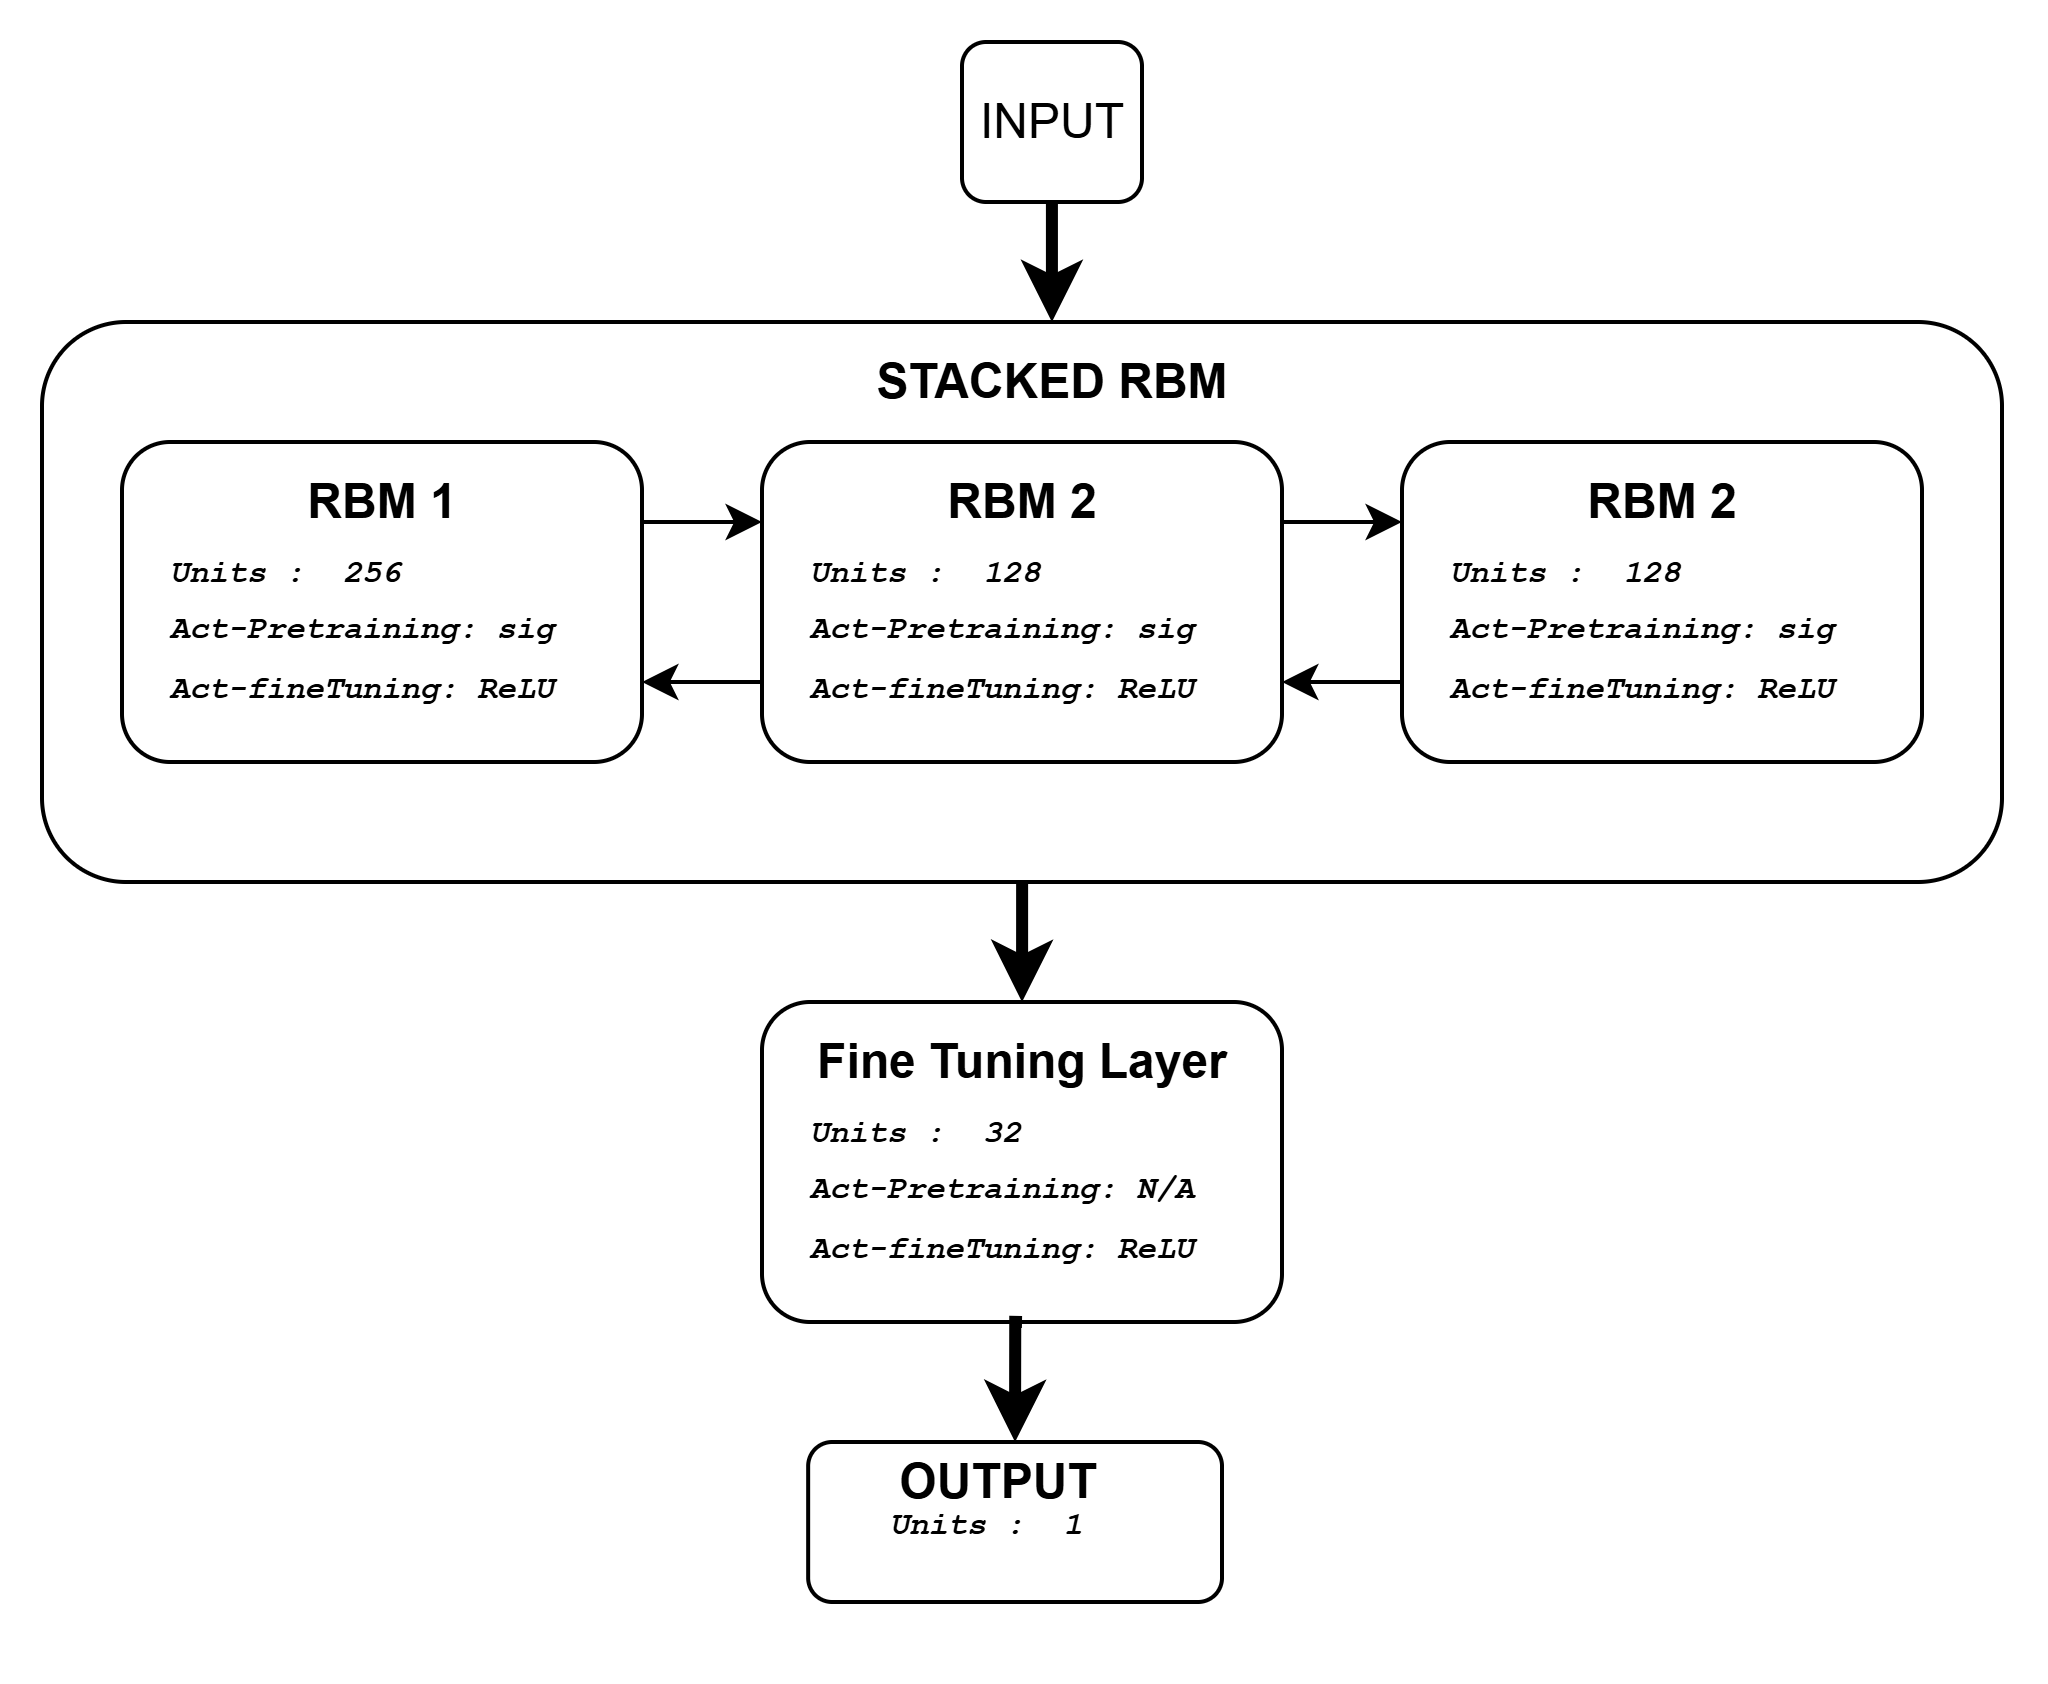
\includegraphics[width=0.7\linewidth]{Chapters/images/DBN_IMPLEMENTATION}
	\caption{Image showing the implementation of the DBN used in the research}
	\label{fig:dbnimplementation}
\end{figure}


\subsubsection{Training Procedure}
 DBN training is split into two sections, unsupervised learning for the RBMs and supervised learning for the stacked RBMs. These procedures will effectively initialize a deep forward network to a good starting point.
 
 \paragraph{Pre-training (Unsupervised)}Each of the RBMs are trained sequentially using the input data in an unsupervised manner to learn a robust and hierarchical representation of the input features. The CD algorithm is used to train each RBM, approximating the gradient using the error equation \ref{eqn:14}. A fixed momentum term of 0.9 is set to accelerate convergence and dampen oscillation.\\ The learning rate was implemented during the pretraining, starting at 0.01 for the first layer and decaying by a factor or 0.8 for each subsequent RBM layer. This decaying factor is to counter the increasing abstraction in higher layer which will require the updates of the layers to be more conservative. Each RBM is trained for 25 epochs, this is because there was a negligible change in the final prediction with increased epochs.
 
 \paragraph{Fine-Tuning (Supervised)} Following the supervised pre-training, the network is unrolled into a standard feed-forward neural network and fine tuned using supervised learning. The learned RBM weights and biases from the pre-training are transferred to initialize the corresponding dense layers in the supervised network. This initialization provides the network with meaningful feature representation. After the transfer the network will learn through supervised learning using standard back-propagation method which will train the network end-to-end.
 \\
 The Adam optimizer is chosen with a base learning rate of 0.001. Adam is preferred over standard SGD for deep learning due to its adaptive learning rates for individual parameters, leading to faster and more stable convergence. The network is then compiled using MSE as its loss function, which is appropriate for regression tasks and is minimized during training.
 
 \paragraph{Regularization Strategies}
 Multiple regularization strategies were employed to prevent overfitting and improve generalization.
 
 \begin{itemize}
 	\item \textbf{L2 Weight Decay} : Applied to the kernel weights of all dense layers with a factor of 0.001 to prevent overfitting by penalizing large weights.
 	\item \textbf{Dropout} : A dropout rate of 0.2 is applied between the hidden layers, and a lower rate (0.1) is applied to the input layer and the final fine-tuning layer to prevent over-reliance on specific neurons.
 	\item \textbf{Early Stopping} : Training terminates if the validation loss) does not improve for 15 consecutive epochs. The best weights corresponding to the lowest validation loss are restored.
 	\item \textbf{Reduce LR On Plateau} : The learning rate is dynamically halved (factor=0.5) if the validation loss plateaus for 8 epochs, ensuring the model can escape local minima.
 \end{itemize}
 
 The DBN was evaluated using three complementary metrics to capture the different aspects of forecasting accuracy. MAPE, MAE and RMSE were used to evaluate and compare the DBN with the other models. These evaluations were performed on inverse transformed predictions to ensure the validation occurred in the original load scale rather than the normalized space used for training. Performance was also assessed separately on both training and test sets to monitor potential overfitting and evaluate generalization capability.
 
 
 
 \subsection{Long Short Term Memory}
 
 LSTM is a specialized type of RNN that is particularly effective for time series data prediction \cite{rafi2021short}1. The LSTM networks are designed to overcome long-term dependency issues such as vanishing and exploding gradients that can occur when processing long data sequences \cite{boopathy2024deep}. The LSTM was chosen for its effectiveness is overcoming long term dependency. 
 
 The LSTM is versatile and also potentially produces more accurate solutions than statistical methods. Since our data is time series data and any prediction thereof should consider past data points to make an accurate prediction make this model a top choice for evaluation.
 
\subsubsection{LSTM Theoretical Background \label{sec:lstm_background}}
 
\paragraph{AN RNN Background} is essential to understand how an LSTM model functions. An RNN is a model that utilizes past sets of information to make a prediction of the present. They achieve this feat by using a feedback loop. The RNN tracks context or previous data on a hidden state at each time step \cite{stryker_ibm_rnn}. This hidden state then works as the memory of the system. 
Imagine \textit{A} is a single unit of the RNN receiving input \textit{$X_t$} , \textit{A} will have a  hidden state \textit{$H_t$} that will store information about the previous input $X_{t-1}$ and it will output \textit{$Y_t$}. Image \ref{fig:rnnsingleunit} adapted from \cite{colah2015understanding} shows how the single unit looks like.

\begin{figure}[h]
	\centering
	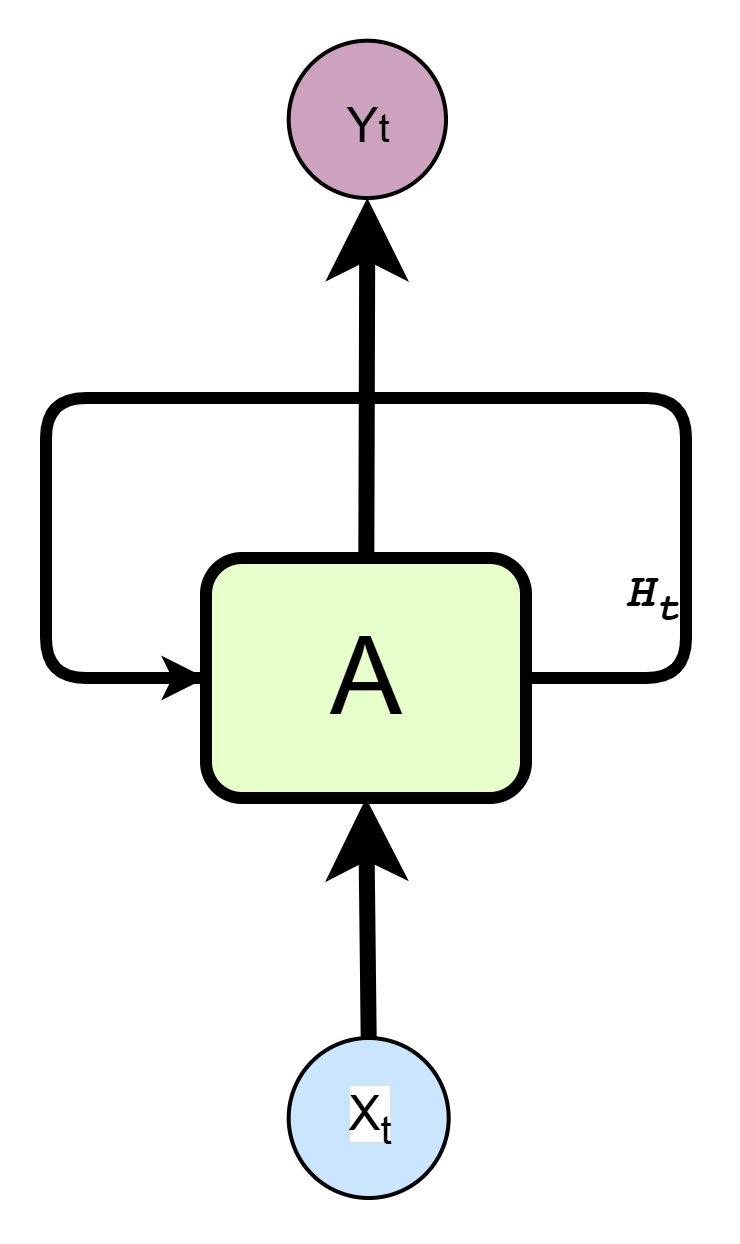
\includegraphics[width=0.1\linewidth]{Chapters/images/rnn_singleunit}
	\caption{A single unit of a recurrent neural network}
	\label{fig:rnnsingleunit}
\end{figure}
If the single unit in figure \ref{fig:rnnsingleunit} is unrolled we will end up with a simple RNN as shown in \ref{fig:unrolledrnn} as adapted from \cite{colah2015understanding}.

\begin{figure}[H]
	\centering
	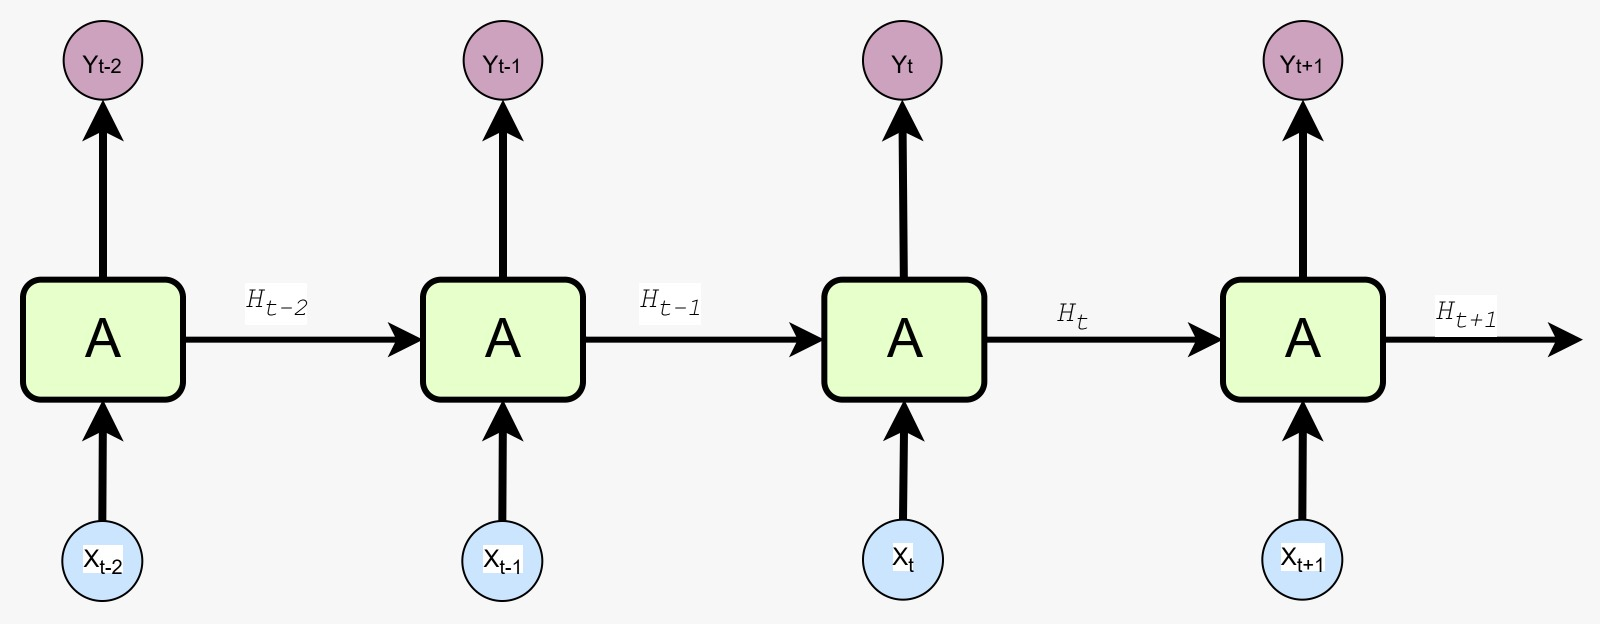
\includegraphics[width=0.5\linewidth,height=0.1\textheight]{Chapters/images/unrolled_rnn.jpeg}
	\caption{An unrolled rnn}
	\label{fig:unrolledrnn}
\end{figure}

An LSTM uses a similar mechanism  to remember past data. It introduces  gates which act as a control mechanism for the what data to keep and discard as we process information. The LSTM has four main components the cell state, forget gate, input gate and output gate. These control the full mechanism of this neural network.

\subsubsection{Cell State}
The cell state is a block of information that propagates all the units of the LSTM. This unit contains the data from previous states that will be used as context in future data cells. \\ 

\begin{figure}[h]
	\centering
	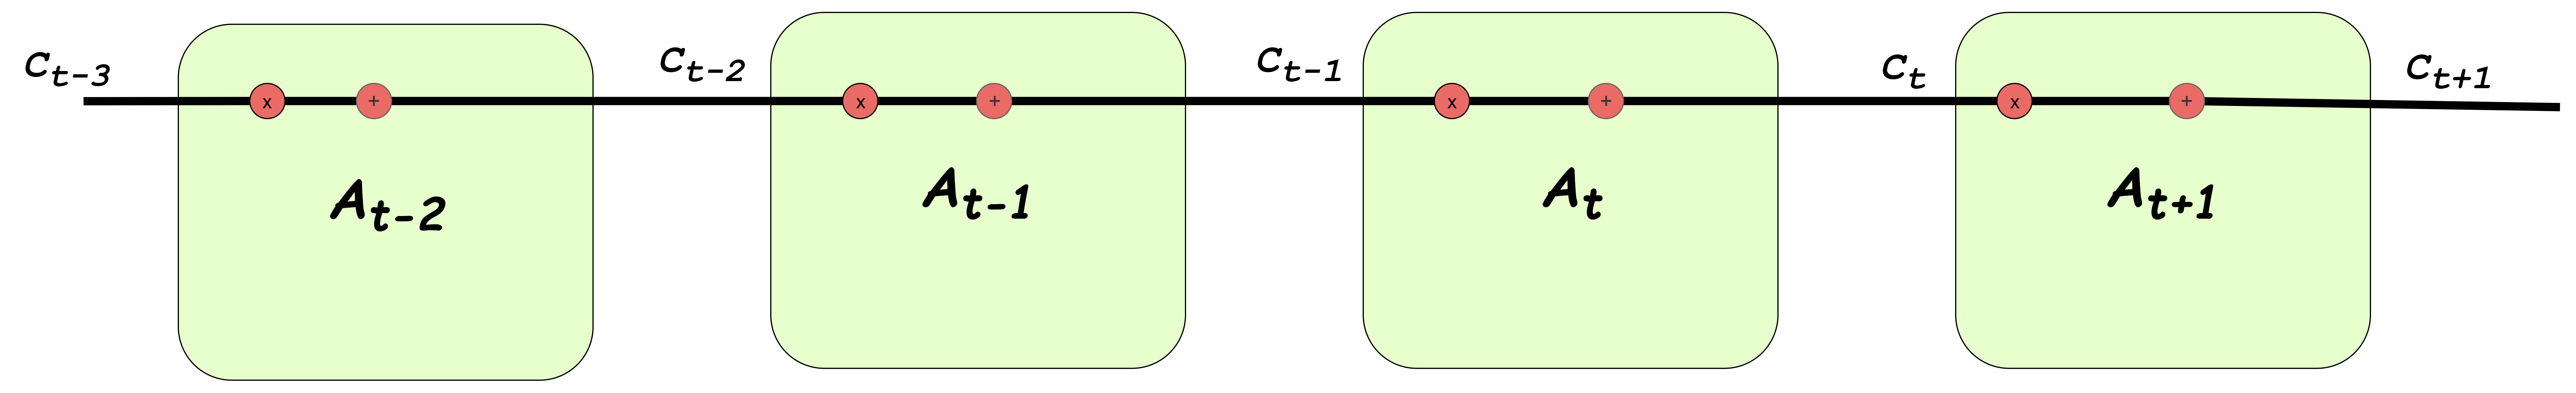
\includegraphics[width=1\linewidth,height=0.1\textwidth]{Chapters/images/cellstate}
	\caption{Cell state propagating through different units of the LSTM carrying data from previous states to future units}
	\label{fig:cellstate}
\end{figure} 

 The image \ref{fig:cellstate} above shows the cell state \textit{$C_{t}$} propagating through the basic unit of an LSTM \textit{$A_t$}. In each of these units through an additive and multiplicative process data is added and removed from the cell state. 
 \paragraph{Forget gate}
 
The cell state contains previous information however there needs to be a way to determine what information is important. The forget gate decides what information to discard from the previous cell state  \textit{$C_{t-1}$} \cite{zhu2025novel}. During back-propagation the forget gate plays a crucial role. If it learns that certain information is important and should be kept for long, the forget gates activation function will be close to 1 and 0 if the information is not very important \cite{zhu2025novel}. Equation \ref{eqn:15}  below adapted from \cite{colah2015understanding} shows how the forget gate works.

\[
f_t = \sigma \Big( W_f \cdot [h_{t-1}, x_t] + b_f \Big)
\tag{23}
\label{eqn:15}
\]
{\small
	\begin{itemize}
		\item $f_t$: Forget gate activation vector at time step $t$ (values between 0 and 1).
		\item $\sigma$: Sigmoid activation function.
		\item $W_f$: Weight matrix for the forget gate.
		\item $[h_{t-1}, x_t]$: Concatenation of the previous hidden state $h_{t-1}$ and the current input $x_t$.
		\item $b_f$: Bias vector for the forget gate.
	\end{itemize}
}

\begin{figure}[h]
	\centering
	\includegraphics[width=0.7\linewidth]{"Chapters/images/LSTM input gate"}
	\caption{Forget gate of an LSTM}
	\label{fig:forgetgate}
\end{figure}
Figure \ref{fig:forgetgate} adapted from \cite{colah2015understanding} shows how the hidden state $h_{t-1}$ and input $x_t$ concatenate together. The concatenated hidden state and input are multiplied with a weight $W_f$ associated with the input.This sigmoid function also has a bias input vector $b_f$ that is added to the weighted hidden state and input .  The two are passed through a sigmoid function using the ReLU activation function giving a number between 0 and 1 as the output. Finally the function $f_t$ is multiplied with $c_{t-1}$ to determine if we add or subtract from the cell state.

\[
C_{t-1}*f_t = 0   ..... \text{    if} f_t = 0 \text{           (forget everything)}
\tag{24.a}
\label{eqn:16.a}
\]

\[
C_{t-1}*f_t = 1  ..... \text{  if} f_t = 1 \text{            (forget nothing)}
\tag{24.b}
\label{eqn:16.b}
\]
 Equation \ref{eqn:16.a} and \ref{eqn:16.b} adapted from \cite{stryker_ibm_rnn} shows how the forget gate will be applied to the cell state through the multiplicative process.
 
 
 \paragraph{Input Gate}
 The input gate determines what new information from the current input and previous hidden state should be stored in the current cell state \cite{rafi2021short}. 
 The input gate quantifies the importance of new data carried in the input \cite{stryker_ibm_rnn}. The input layer is split into two parts, the output of the input gate $i_t$ and a candidate cell state $\tilde{C_t}$ used to update the global cell state. $\tilde{C_t}$ allows retaining of important information and effectively updating the global cell state \cite{zhu2025novel}.
\begin{figure}[h]
	\centering
	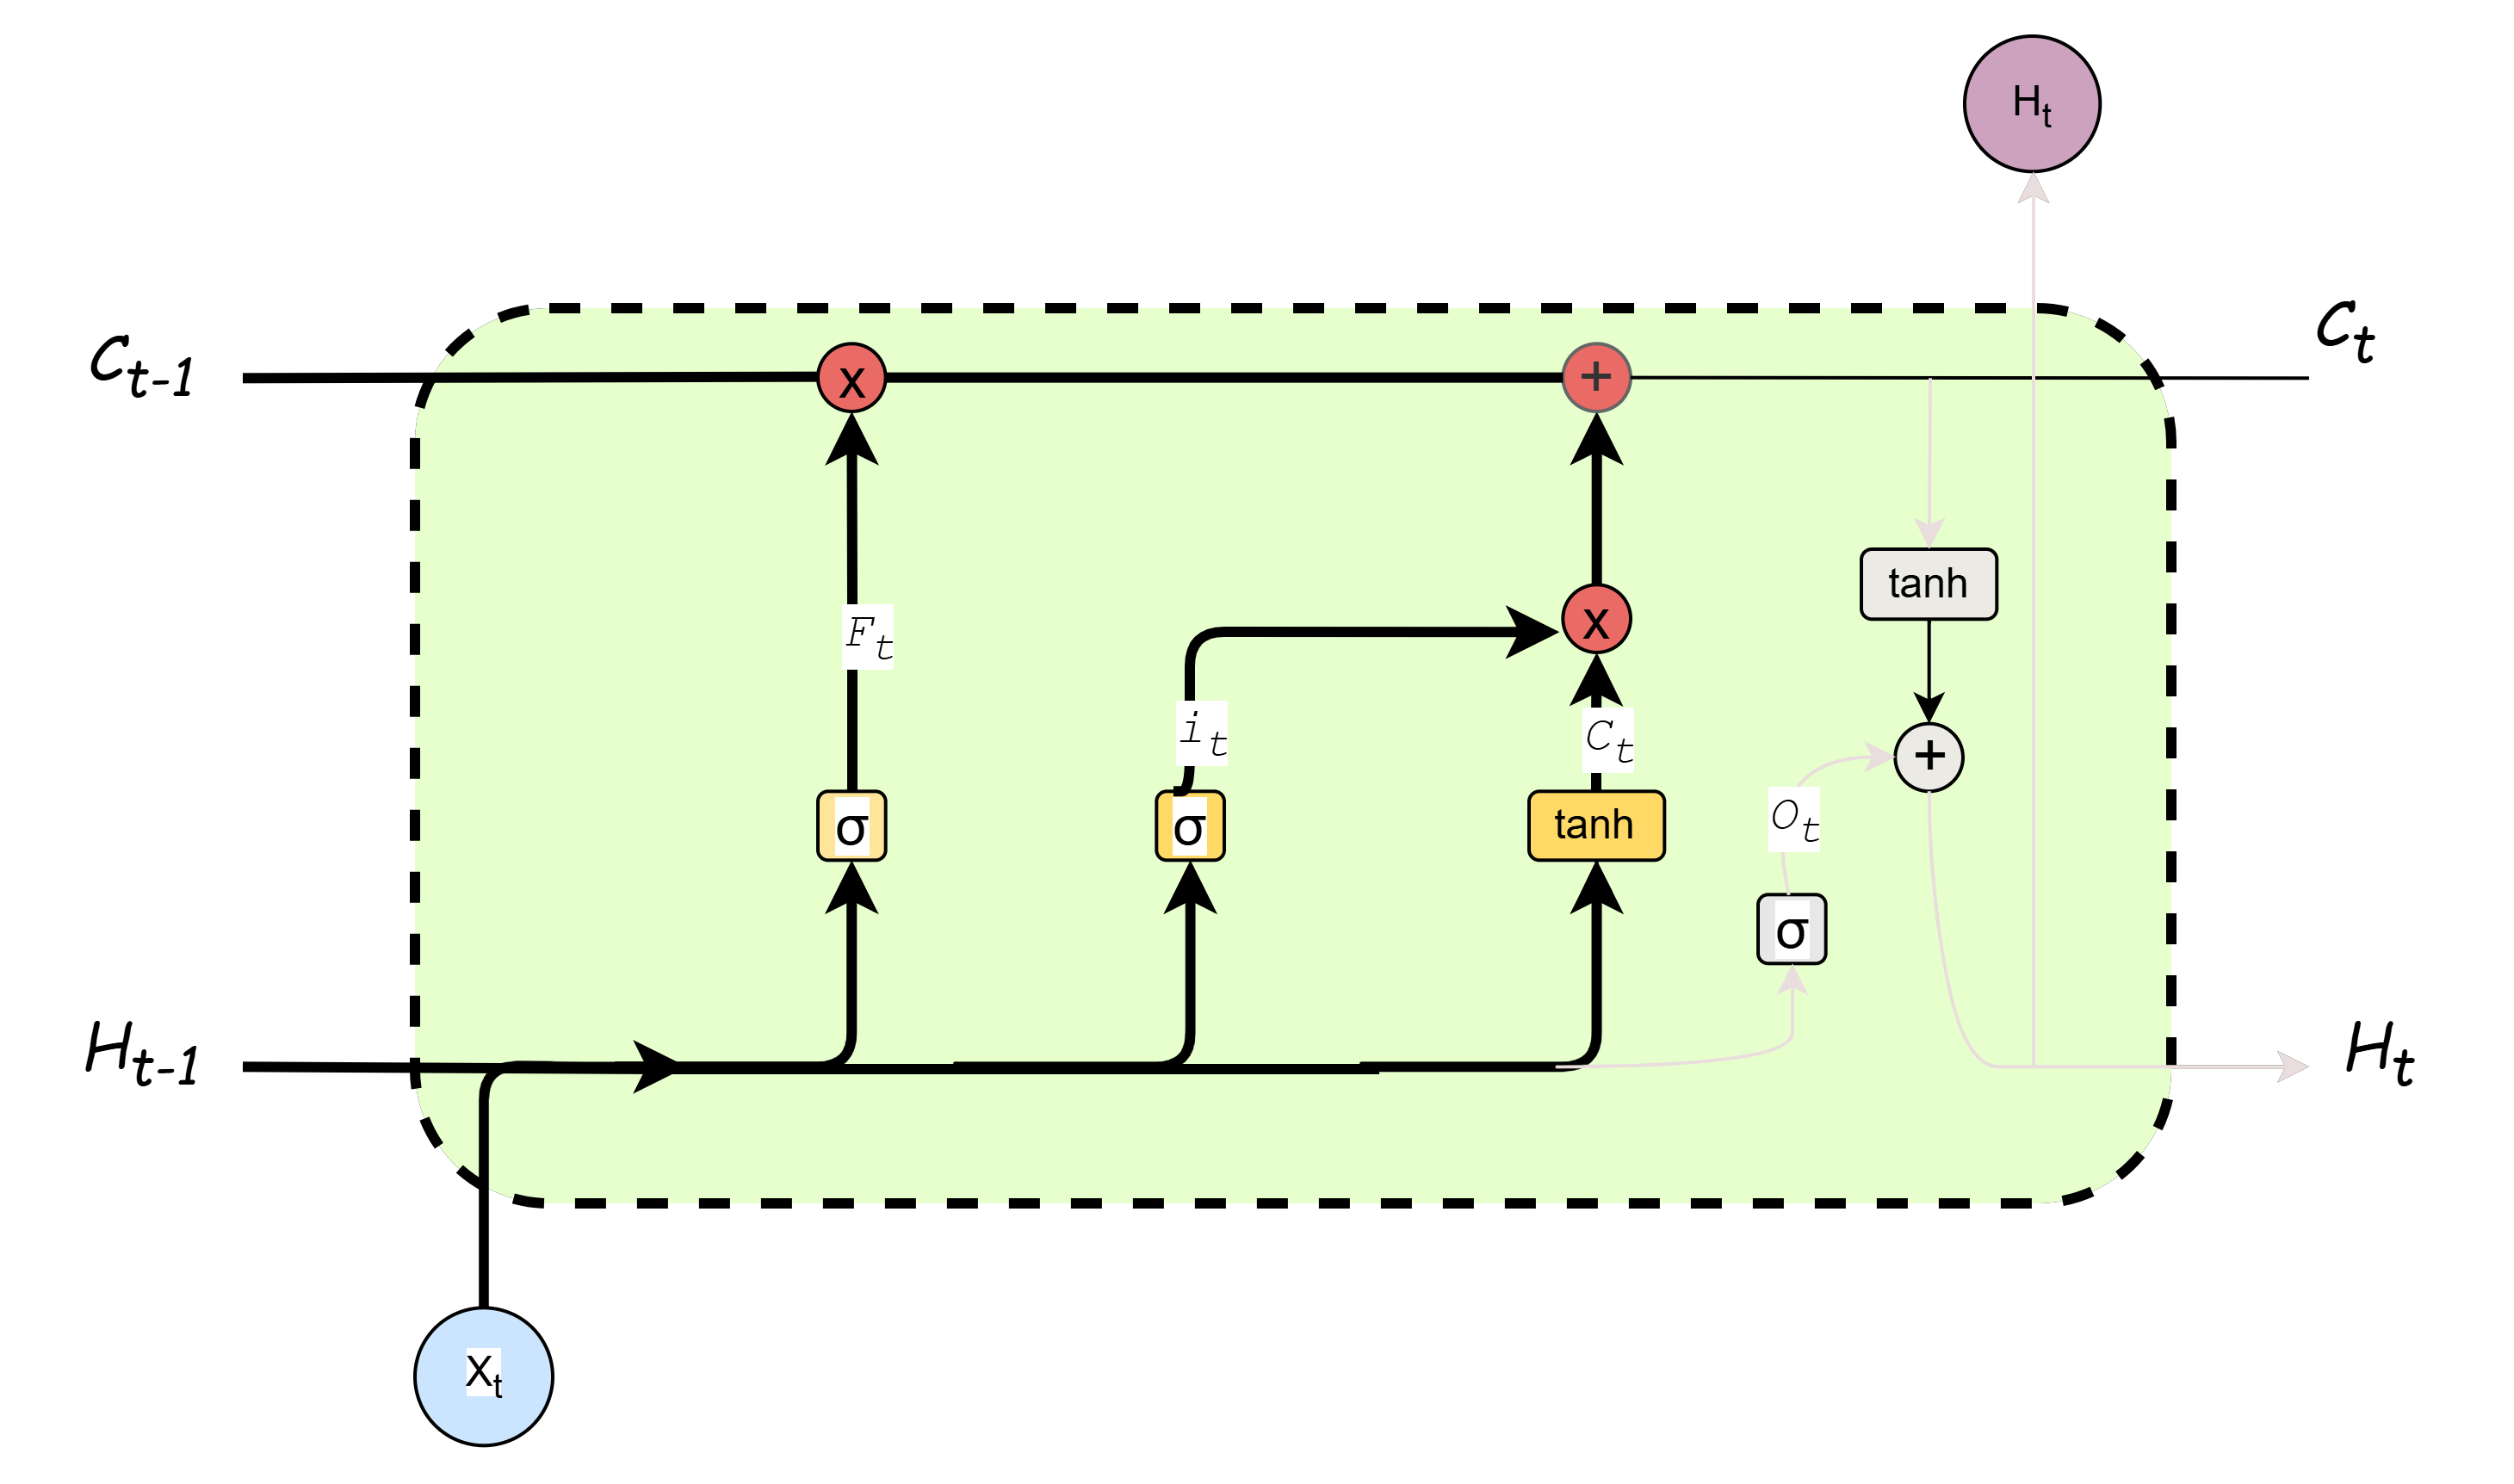
\includegraphics[width=0.7\linewidth]{Chapters/images/forget_inputgates}
	\caption{An LSTM unit with the forget and input gate }
	\label{fig:forgetinputgates}
\end{figure}

Figure \ref{fig:forgetinputgates} shows how the forget and input gates. Below are the equations that determine the functionality of the input gate. % Input gate equation
\[
i_t = \sigma \Big( W_i \cdot [h_{t-1}, x_t] + b_i \Big)
\tag{25}
\label{eqn:inputgate}
\]

% Candidate cell state
\[
\tilde{C}_t = \tanh \Big( W_c \cdot [h_{t-1}, x_t] + b_c \Big)
\tag{26}
\label{eqn:candidatecell}
\]

% Cell state update
\[
C_t = f_t \odot C_{t-1} + i_t \odot \tilde{C}_t
\tag{27}
\label{eqn:cellupdate}
\]
{\small
\begin{itemize}
	\item $i_t$: Input gate output at time step $t$.
	\item $\sigma$: Sigmoid activation function.
	\item $W_i, W_c$: Weight matrices for the input gate and candidate cell state.

	\item $b_i, b_c$: Bias vectors for the input gate and candidate cell state.
	\item $\tilde{C}_t$: Candidate cell state (potential new memory).
	\item $\tanh$: Hyperbolic tangent activation function.
	\item $C_t$: Updated cell state at time step $t$.
	\item $f_t$: Forget gate activation vector at time step $t$.
	\item $C_{t-1}$: Previous cell state.
	\item $\odot$: Element-wise product.
\end{itemize}
}
As shown in figure \ref{fig:forgetinputgates} the candidate cell state and the input output gate are combined through an element wise multiplication. The global cell state is also updated by using an additive operation of the forget gate output and the output of the multiplication in the input gate.
 \paragraph{Output Gate}
The output gate determines what information from the cell state should be passed onto the hidden state \cite{zhu2025novel}. The hidden state acts as the output of the unit of processing and will also be used in the following units of processing.
 
 Figure \ref{fig:forgetinputoutputgates1} shows the complete unit of processing with the output gate. The hidden state takes a sigmoid processed concatenated $h_{t-1}$ and $x_t$ with a tanh processed $C_t$ the output will be through a multiplicative output. 
 % Output gate equation
 \[
 o_t = \sigma \Big( W_o \cdot [h_{t-1}, x_t] + b_o \Big)
 \tag{28}
 \label{eqn:outputgate}
 \]
 % Hidden state update
 \[
 h_t = o_t \odot \tanh(C_t)
 \tag{29}
 \label{eqn:hiddenstate}
 \]
 {\small 
 \begin{itemize}
 	\item $o_t$: Output gate activation vector at time step $t$.
 	\item $W_o$: Weight matrix for the output gate.
 	\item $b_o$: Bias vector for the output gate.
 	\item $h_t$: Hidden state at time step $t$ (output of the LSTM block).
 	\item $C_t$: Updated cell state at time step $t$.
 	\item $\tanh$: Hyperbolic tangent activation function.
 \end{itemize}
}
 \begin{figure}[h]
 	\centering
 	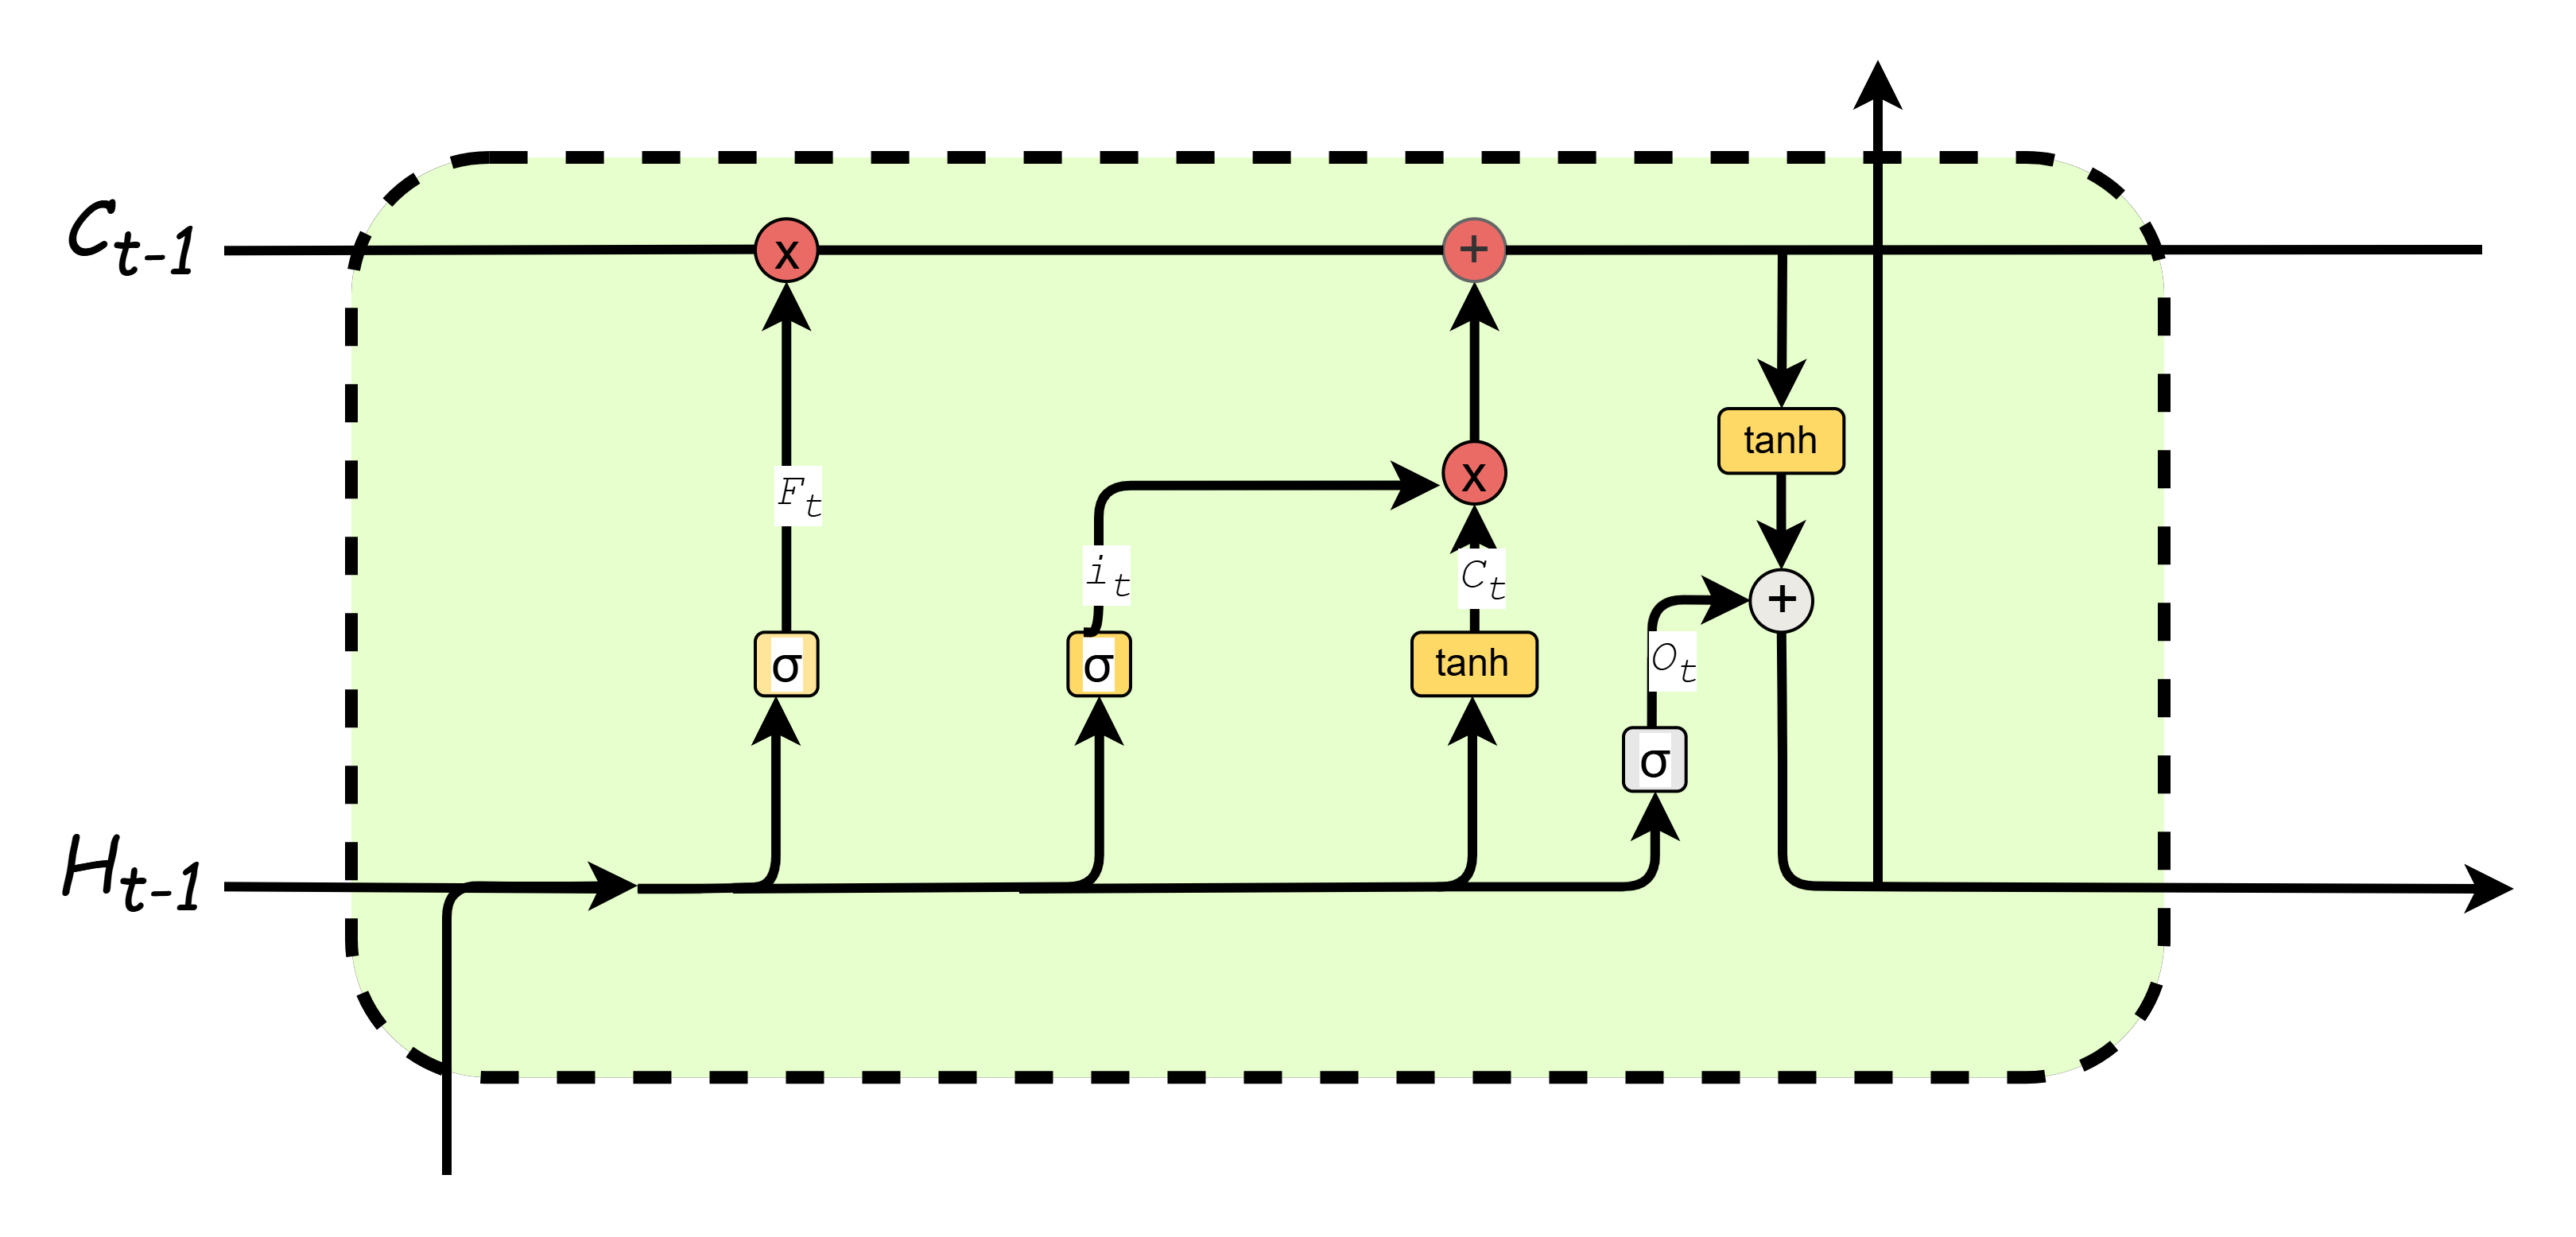
\includegraphics[width=0.5\linewidth]{Chapters/images/forget_input_output_gates1}
 	\caption{Complete LSTM unit with forget, input and output gates }
 	\label{fig:forgetinputoutputgates1}
 \end{figure}
  Equation \ref{eqn:outputgate}  shows the combination for the output and \ref{eqn:hiddenstate} shows the output of the LSTM unit.
  
  A combination of the three gates and their interaction of the cell state form a single unit for an LSTM network. Figure \ref{fig:full-lstm} shows multiple units of an LSTM and how they relate to each other in a neural network. 
 \begin{figure}[h]
 	\centering
 	\includegraphics[width=0.9\linewidth]{"Chapters/images/full lstm"}
 	\caption{full lstm}
 	\label{fig:full-lstm}
 \end{figure}
 The LSTM model uses the power of remembering past data and filtering out important and unnecessary data to the given task to make predictions. In STLF a model capable of finding the important data points in past data to predict for a future data point is crucial. The LSTM model perfects remembrance through its cell state and gate system making it effective for STLF.
 
 \subsubsection{LSTM Architecture for STLF}
 
 The architecture for the LSTM model used in this research used tensorflow and scikitlearn frameworks to build and train the models. The model followed the same data preprocessing procedures mentioned in section \ref{sec:datapreprocessing}. In addition to the data pre-processing steps a lag feature was added for the STLF. LSTM requires past data to make an accurate prediction and by adding lag features to the data helps the model train with context of the past data. The lag features included the past demand values at 1-hour, 24-hours and 168-hours intervals. Introduction of lag features ensured that the model had access tp both short term and long term temporal dependencies. The dataset was further split into 80\% training and 20\% testing subsets, to monitor the models generalization.
 
 \subsubsection{Sequence Formation}
 The input of the LSTM model was reshaped into sequences of historical observation to future forecasts.
 {\small
 \begin{itemize}
 	\item \textbf{Input sequence length} : 168 hours (7 days)
 	\item \textbf{Forecast Horizon} : 24 hours (1 day)
 \end{itemize}
}
 Each training instance therefore contained 168 past observations of all features as input and the next 24-hours of demand as the target output. All the rows containing missing values introduced by lag and rolling operations were removed.
 
 \subsubsection{Model Architecture}
 
 The proposed LSTM model was created using a stacked architecture to capture short and long term dependencies in the time series data. The architecture comprised: 
 {\small 
 \begin{itemize}
 	\item \textbf{LSTM Layer 1}: 128 units followed by batch normalization and 20\% dropout.
 	\item \textbf{LSTM Layer 2}: 64 units with Batch Normalization and 20\% Dropout.
 	
 	\item\textbf{LSTM Layer 3}: 32 units with Batch Normalization and 10\% Dropout.
 	
 	\item \textbf{Dense Layer}: 50 neurons with ReLU activation and 10\% Dropout.
 	
   \item\textbf{ Output Layer}: Linear activation with 24 neurons, corresponding to the 24-hour forecast horizon.
 \end{itemize}
}
 
 The model was compiled using the Adam optimizer with a learning rate of 0.001 and trained to minimize the MSE loss function. The MAE was tracked as a secondary performance metric.
 
 \subsubsection{Model Training}The model was trained on the prepared training set with followed parameters.
 {\small
 \begin{itemize}
 	\item \textbf{Epochs}:  50-100
 	\item \textbf{Batch Size}:  32
 	\item\textbf{Validation split} : 0.2
 	\end{itemize}
 }
 	In order to better convergence and prevent overfitting of the model we used call back methods. 
 {\small
 		\begin{itemize}
 		\item \textbf{EarlyStopping} with a  15 epochs stopping patience and best model restoration.
 		\item \textbf{ReduceLROnPlateau} to dynamically reduce the learning rate upon validation loss stagnation.
 		\item \textbf{ModelCheckpoint} to save the model automatically with the lowest validation loss.
 	\end{itemize} }
 Training progress was monitored through loss and MAE curves for training and validations sets. The model was evaluated using the evaluation metrics mentioned in section \ref{sec:eval_metrics}.
 	
Flowchart \ref{fig:lstmflowchart} in appendix A shows a clear methodology followed to make the LSTM model. This methodology ensured a systematic approach to implementing an LSTM-based forecasting framework, emphasizing robust feature engineering, careful data preprocessing, and a well-regularized deep learning model architecture optimized for temporal sequence learning.


\subsection{Hybrid Model : CNN-LSTM }
A CNN-LSTM hybrid model is a deep learning architecture designed to combine the strengths of Convolutional Neural Networks (CNN) and LSTM networks, typically to enhance forecasting accuracy and handle complex, non-linear time series data, such as electrical load data sequences \cite{zhu2025novel}. The model takes advantage of the CNNs capability of feature extraction and the LSTMs ability to capability to extract sequence patterns and long-short term dependencies \cite{alhussein2020hybrid}. The LSTM theoretical background was covered in section \ref{sec:lstm_background}, therefore we will only look at the theoretical background of a CNN.

\subsubsection{CNN Theoretical Background}

A CNN is considered the most representative neural network, this is because of its inspiration by biological nervous systems such as the brain \cite{o2015introduction}. A CNN is composed of neurons that self optimize through learning \cite{o2015introduction}.Their architecture is formed by stacking three primary types of layers:

\paragraph{Convolutional Layer :} This is the fundamental component that perform feature extraction using learnable kernels or filters \cite{yamashita2018convolutional}. The kernels are usually small spatial dimensions but extend themselves across their entire depth of the input volume \cite{ajit2020review}. The kernels themselves are optimizable feature extractors, containing sets of learnable parameters \cite{yamashita2018convolutional}.

The layer convolves each filter across the dimensions of the input volume. This is a specialized type of linear operation. As the kernel glides over the input, the scalar product  between the kernel's weights and the local region of the input volume is calculated and summed to obtain a single output value.

\paragraph{Activation Layer with  Rectified linear Unit} layer is usually applied to every element after the convolution function \cite{o2015introduction}.The purpose of the ReLU is to introduce non-linearity into the network, which is essential because of the highly non linear format of the data CNN's process \cite{wu2017introduction}. The ReLU equation \ref{eqn:23} as adapted from \cite{wu2017introduction}.
\[
f_t = \max (0,x)
\tag{30}
\label{eqn:23}
\]
\paragraph{Pooling Layers} aim to gradually reduce the dimensionality of the representation, subsequently lowering the number of parameters and the model's computational complexity \cite{li2021survey}. In simple terms it reduces the size of the feature maps while keeping the most important information. The most common type of pooling is \textit{Max Pooling}, which takes the maximum value from each window of the output  which in turn helps in reduction of computation and overfitting.

\paragraph{Fully Connected Layer} is the layer that performs the classification task in a CNN \cite{IBM_WhatAreCNNs_2025}. This will be based on the features that are extracted in the pooling and convolutional layers. This layer performs as a standard neural network, producing class scores from activation \cite{o2015introduction}.

Figure \ref{fig:cnn} is the architecture of a CNN as adapted from \cite{o2015introduction}.
\begin{figure}[H]
	\centering
	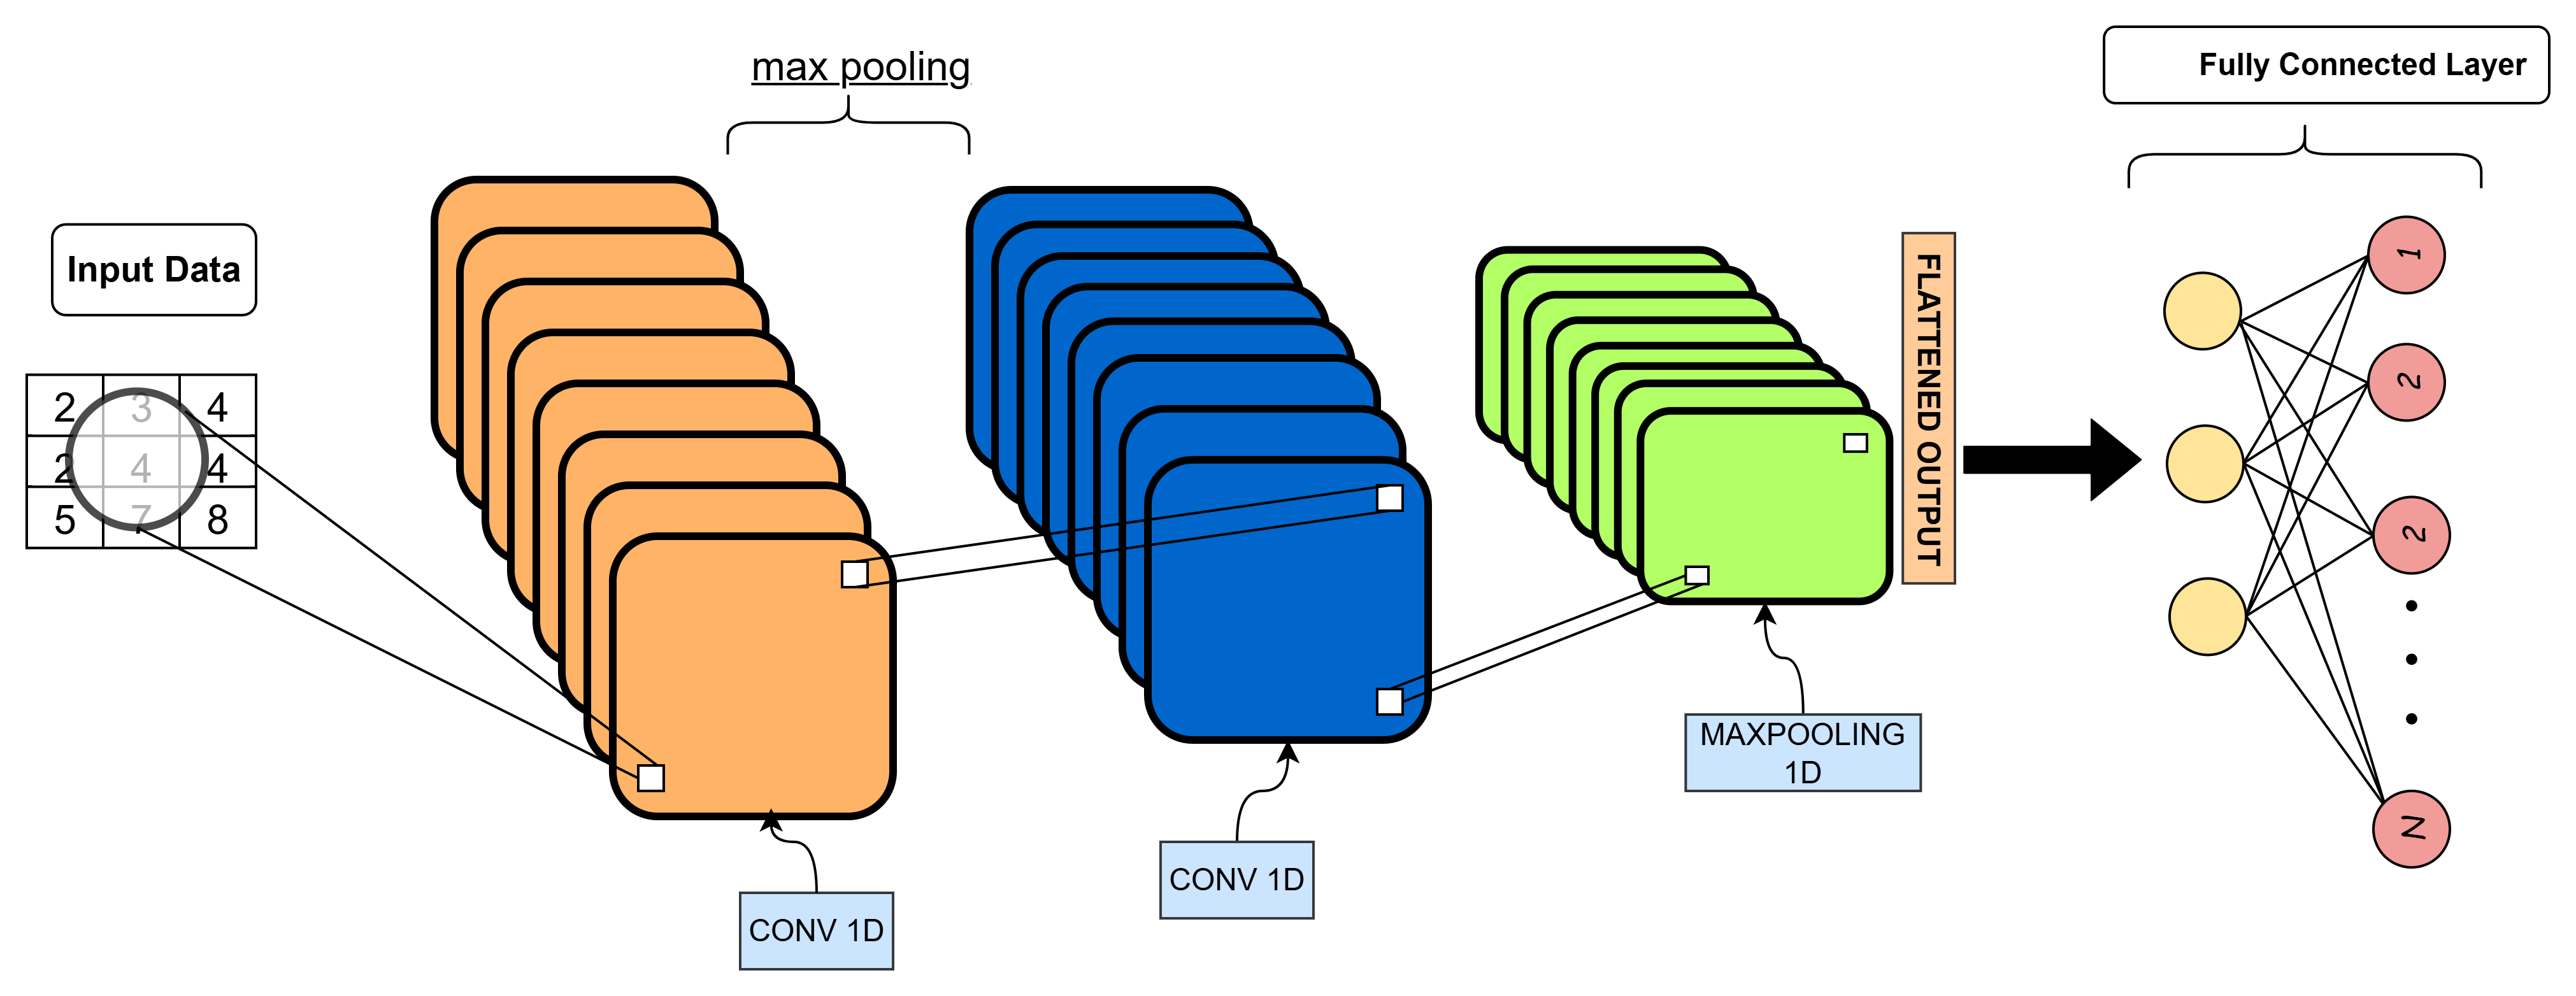
\includegraphics[width=0.7\linewidth]{Chapters/images/CNN}
	\caption{An illustration of the CNN model}
	\label{fig:cnn}
\end{figure}


\subsubsection{CNN-LSTM Architecture and Methodology}

\subsubsection{Data Preparation and Framing}
This model uses the continuous\_dataset.csv converted into pandas, this is to maintaining uniformity across the different models tested. The data is processed following the steps mentioned in section \ref{sec:datapreprocessing}. Adding onto the already extensive data processing a \textit{lookback window} of 168 hours was used to predict the next 24-hours which is the forecast horizon. This means that each input consisted of 168 hourly observations while the corresponding label contained the next 24 hourly demand values.

\subsubsection{Constructing Multi Step Time series}
In order to model multi hour ahead forecast, a sliding window approach was used to construct the input output pairs. For every time step \textit{t} an input matrix\\ \[
X_t =[x_{t-167},x_{t-166}, ... , x_t]
\] \\
 was created to predict the target vector \\
 \[
 y_t = [y_{t+1},y_{t+2}, ... , y_{t+24}] 
 \]
corresponding to the next 24 hours.This process generated overlapping input–output pairs that captured both short-term fluctuations and weekly seasonal patterns. The resulting sequences were reshaped into the three-dimensional format 
\textit{(samples,timesteps,features)} required for deep learning models in TensorFlow.
\subsubsection{CNN-LSTM Model Architecture}
The proposed model combines a CNN and LSTM as implemented by \cite{rafi2021short}. The CNN layers act as feature extractors while the LSTM capture the longer term temporal relationships. The dense layers are used to integrate the learned features and generate multi-step forecasts for the next 24 hours.
{\small
\begin{itemize}
	\item \textbf{CNN Block}   \begin{itemize}
		\item 64 filter Layer 1-D Convolutional layer
		\item 32 filter Layer 1-D Convolutional layer
		\item Kernel size = 3 , Padding = 3 (for temporal dimension preservation)
		\item ReLU Activation 
		\item MaxPooling 1D layer
		\item Dropout rate =  0.2 (enhances generalization)
	\end{itemize}
	\item \textbf{LSTM Block} \begin{itemize}
		\item 50 unit Layer 1 for hierarchical feature extraction
		\item 50 unit Layer 2 for sequential output and passes its representation to dense layers.
		\item Dropout rate = 0.2 also used between layers for enhanced generalization.
	\end{itemize}
	\item \textbf{Dense Layers (Fully Connected Block)}  \begin{itemize}
		\item 64 neuron Dense layers with RelU activation
		\item Dropout layer for reduction of overfitting
		\item 32 neuron Dense layer
		\item 24 neuron Output layer , with each neuron corresponding to a forecasted hour.
	\end{itemize}
\end{itemize}}
\begin{figure}[h]
	\centering
	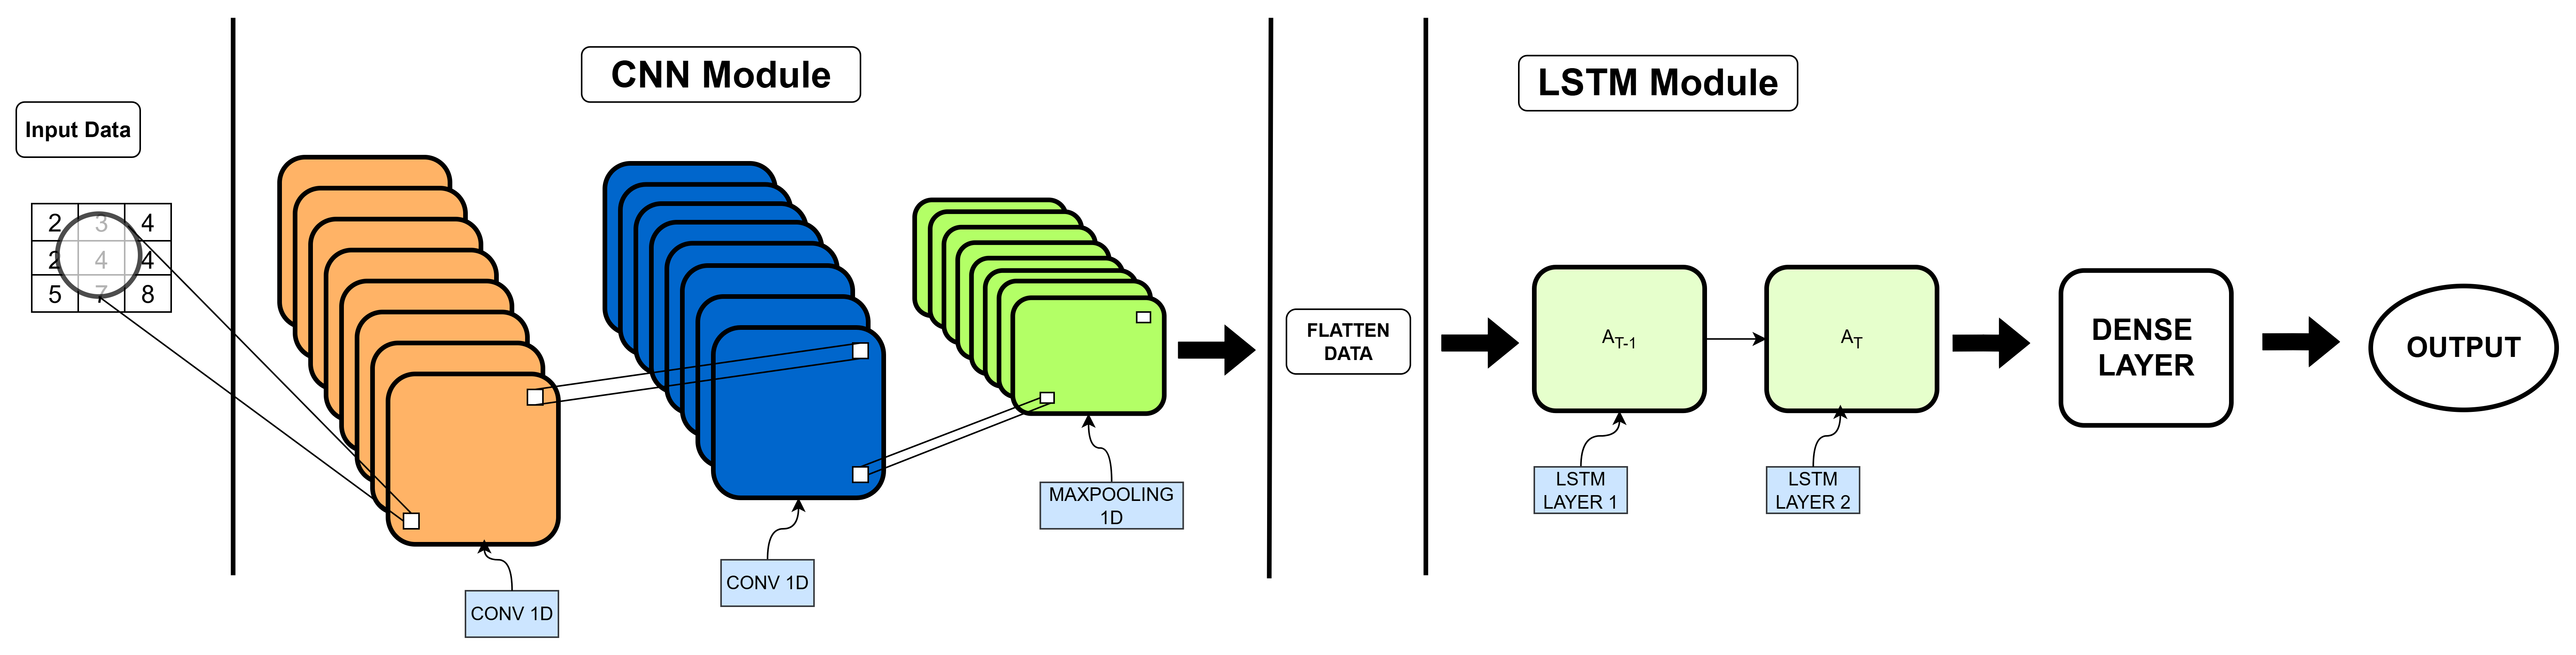
\includegraphics[width=\linewidth]{Chapters/images/CNN-LSTM}
	\caption{Illustration of the CNN-LSTM hybrid model with 2 CNN layers and 2 LSTM layer and a dense layer that produces the output}
	\label{fig:cnn-lstm}
\end{figure}
The model was compiled with the Adam Optimizer with a learning rate of 0.001. MAE, MAPE, MSE were used as performance metrics to evaluate the model. Figure \ref{fig:cnn-lstm} illustrates the cnn-lstm hybrid model as adapted from \cite{rafi2021short}.
\subsubsection{Model Training and Validation}
The CNN-LSTM model was trained on an 80/20 split train/test split. Training was run for 100 epochs with a batch size of 32. We use two callback functions to improve performance.
{\small
\begin{itemize}
	\item \textbf{EarlyStopping:} Monitored validation loss and halted training when no improvement was observed for 15 consecutive epochs, restoring the best weights.
	\item \textbf{ReduceLROnPlateau:} Reduced the learning rate by a factor of 0.5 if validation loss plateaued for five epochs, preventing overfitting and ensuring stable convergence.
\end{itemize}}
The training and validation losses were plotted to monitor model convergence and ensure that the model generalized well to unseen data. The callback functions helped in ensuring that our computational resources- are not wasted during the training of the models.
































